\documentclass{beamer}
\usepackage{ctex, hyperref}
\usepackage[T1]{fontenc}
\usefonttheme[onlymath]{serif}
\usepackage{latexsym,amsmath,xcolor,multicol,booktabs,calligra}
\usepackage{graphicx,pstricks,listings,stackengine}
\usepackage{multirow}

\definecolor{deepblue}{rgb}{0,0,0.5}
\definecolor{deepred}{rgb}{0.6,0,0}
\definecolor{deepgreen}{rgb}{0,0.5,0}

\graphicspath{{../images/}{pic/}}

\author{韦康琦}
\title{面向移动端双目的轻量化\\三维人体姿态估计方法研究}
\subtitle{硕士学位论文答辩}
\institute{中南大学计算机学院\\指导教师：张德宇教授}
\date{2026年4月}
\usepackage{CSU}
\setbeamertemplate{navigation symbols}{}

\begin{document}

\kaishu
\begin{frame}
    \titlepage
    \begin{figure}[htpb]
        \begin{center}
            
\includegraphics[width=0.15\linewidth]{pic/Central_South_University_Logo.eps}
        \end{center}
    \end{figure}
\end{frame}

\begin{frame}{目录}
    \tableofcontents[sectionstyle=show,subsectionstyle=show/shaded/hide]
\end{frame}


%% ========================================
\section{研究背景与意义}
%% ========================================

\begin{frame}{研究背景}
    \begin{columns}[T]
        \begin{column}{0.50\textwidth}
            \small
            \begin{itemize}
                \item 三维人体姿态估计是视觉感知与行为理解的基础能力
                \item 移动机器人、安防、VR/AR 要求\textbf{空间精度}与\textbf{端侧实时性}并重
                \item 手机、机器人、头显普遍配备\textbf{双摄模组}，双目几何信息唾手可得
            \end{itemize}
            \vspace{2pt}
            \begin{exampleblock}{\small 典型端侧双目设备}
                \centering
                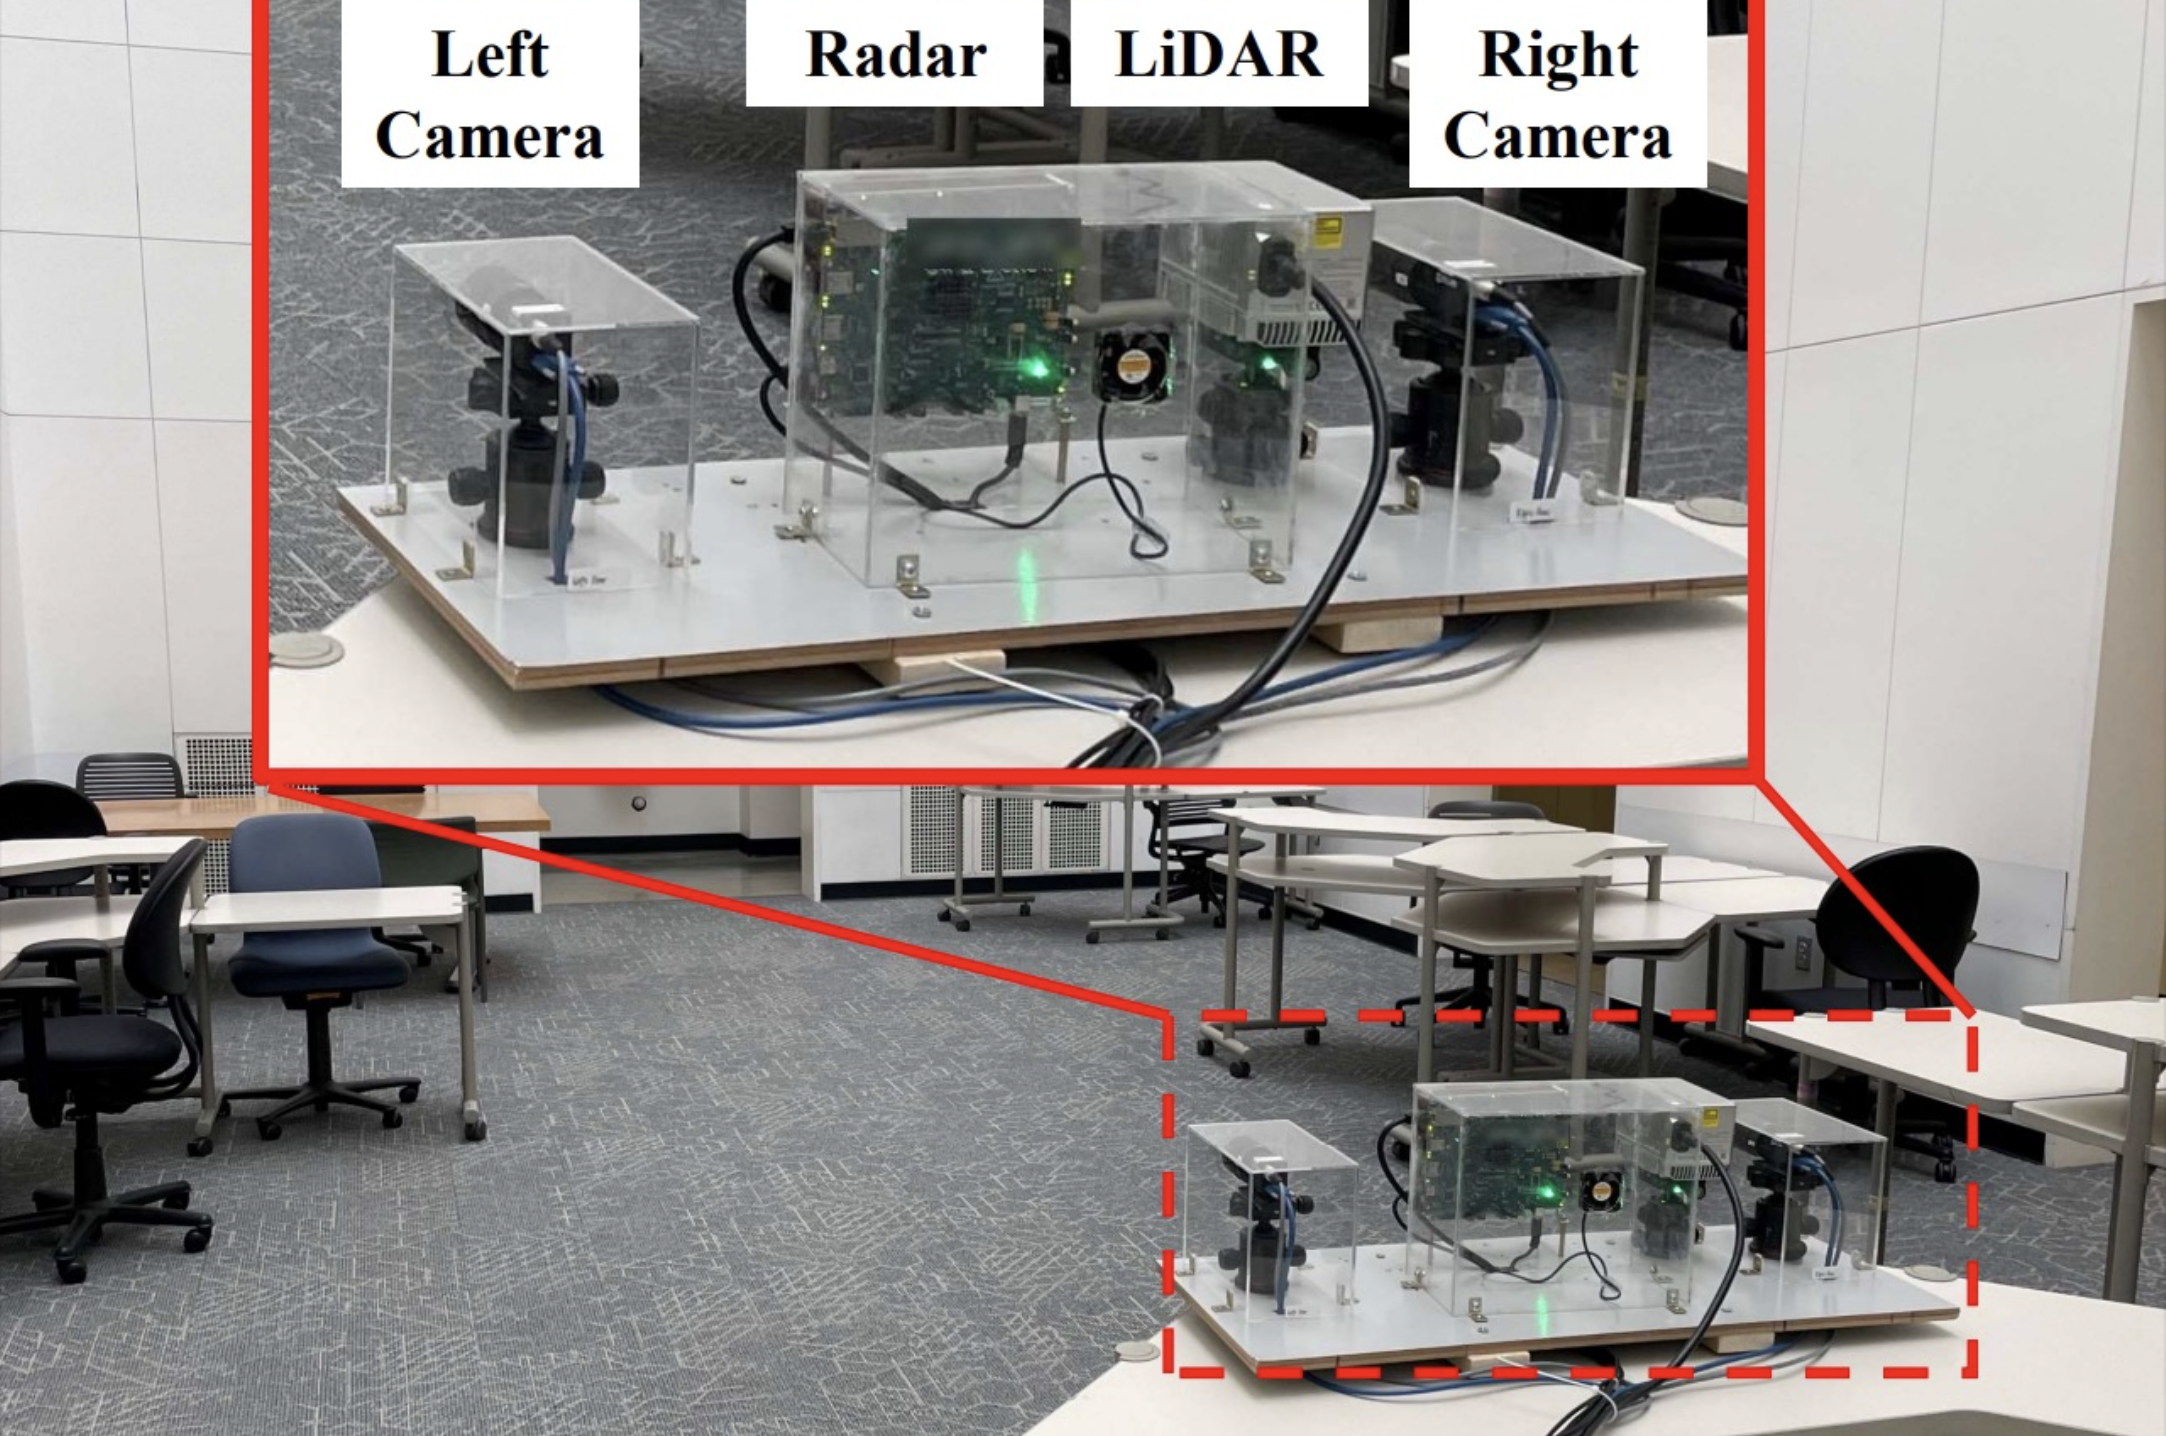
\includegraphics[width=0.9\linewidth,height=2.4cm,keepaspectratio]{device.png}
            \end{exampleblock}
        \end{column}
        \begin{column}{0.47\textwidth}
            {\centering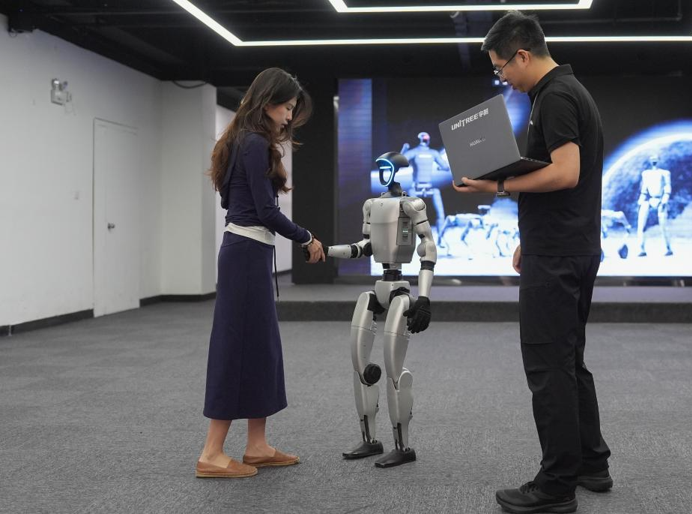
\includegraphics[width=\linewidth,height=5.5cm,keepaspectratio]{Human_computer_interaction_scenario.png}\\[2pt]
            \footnotesize 机器人与人交互场景\par}
        \end{column}
    \end{columns}
\end{frame}

\begin{frame}{问题分析：三大挑战}
    \begin{columns}[T]
        \begin{column}{0.48\textwidth}
            \begin{block}{\small ① 单目深度歧义}
                \centering
                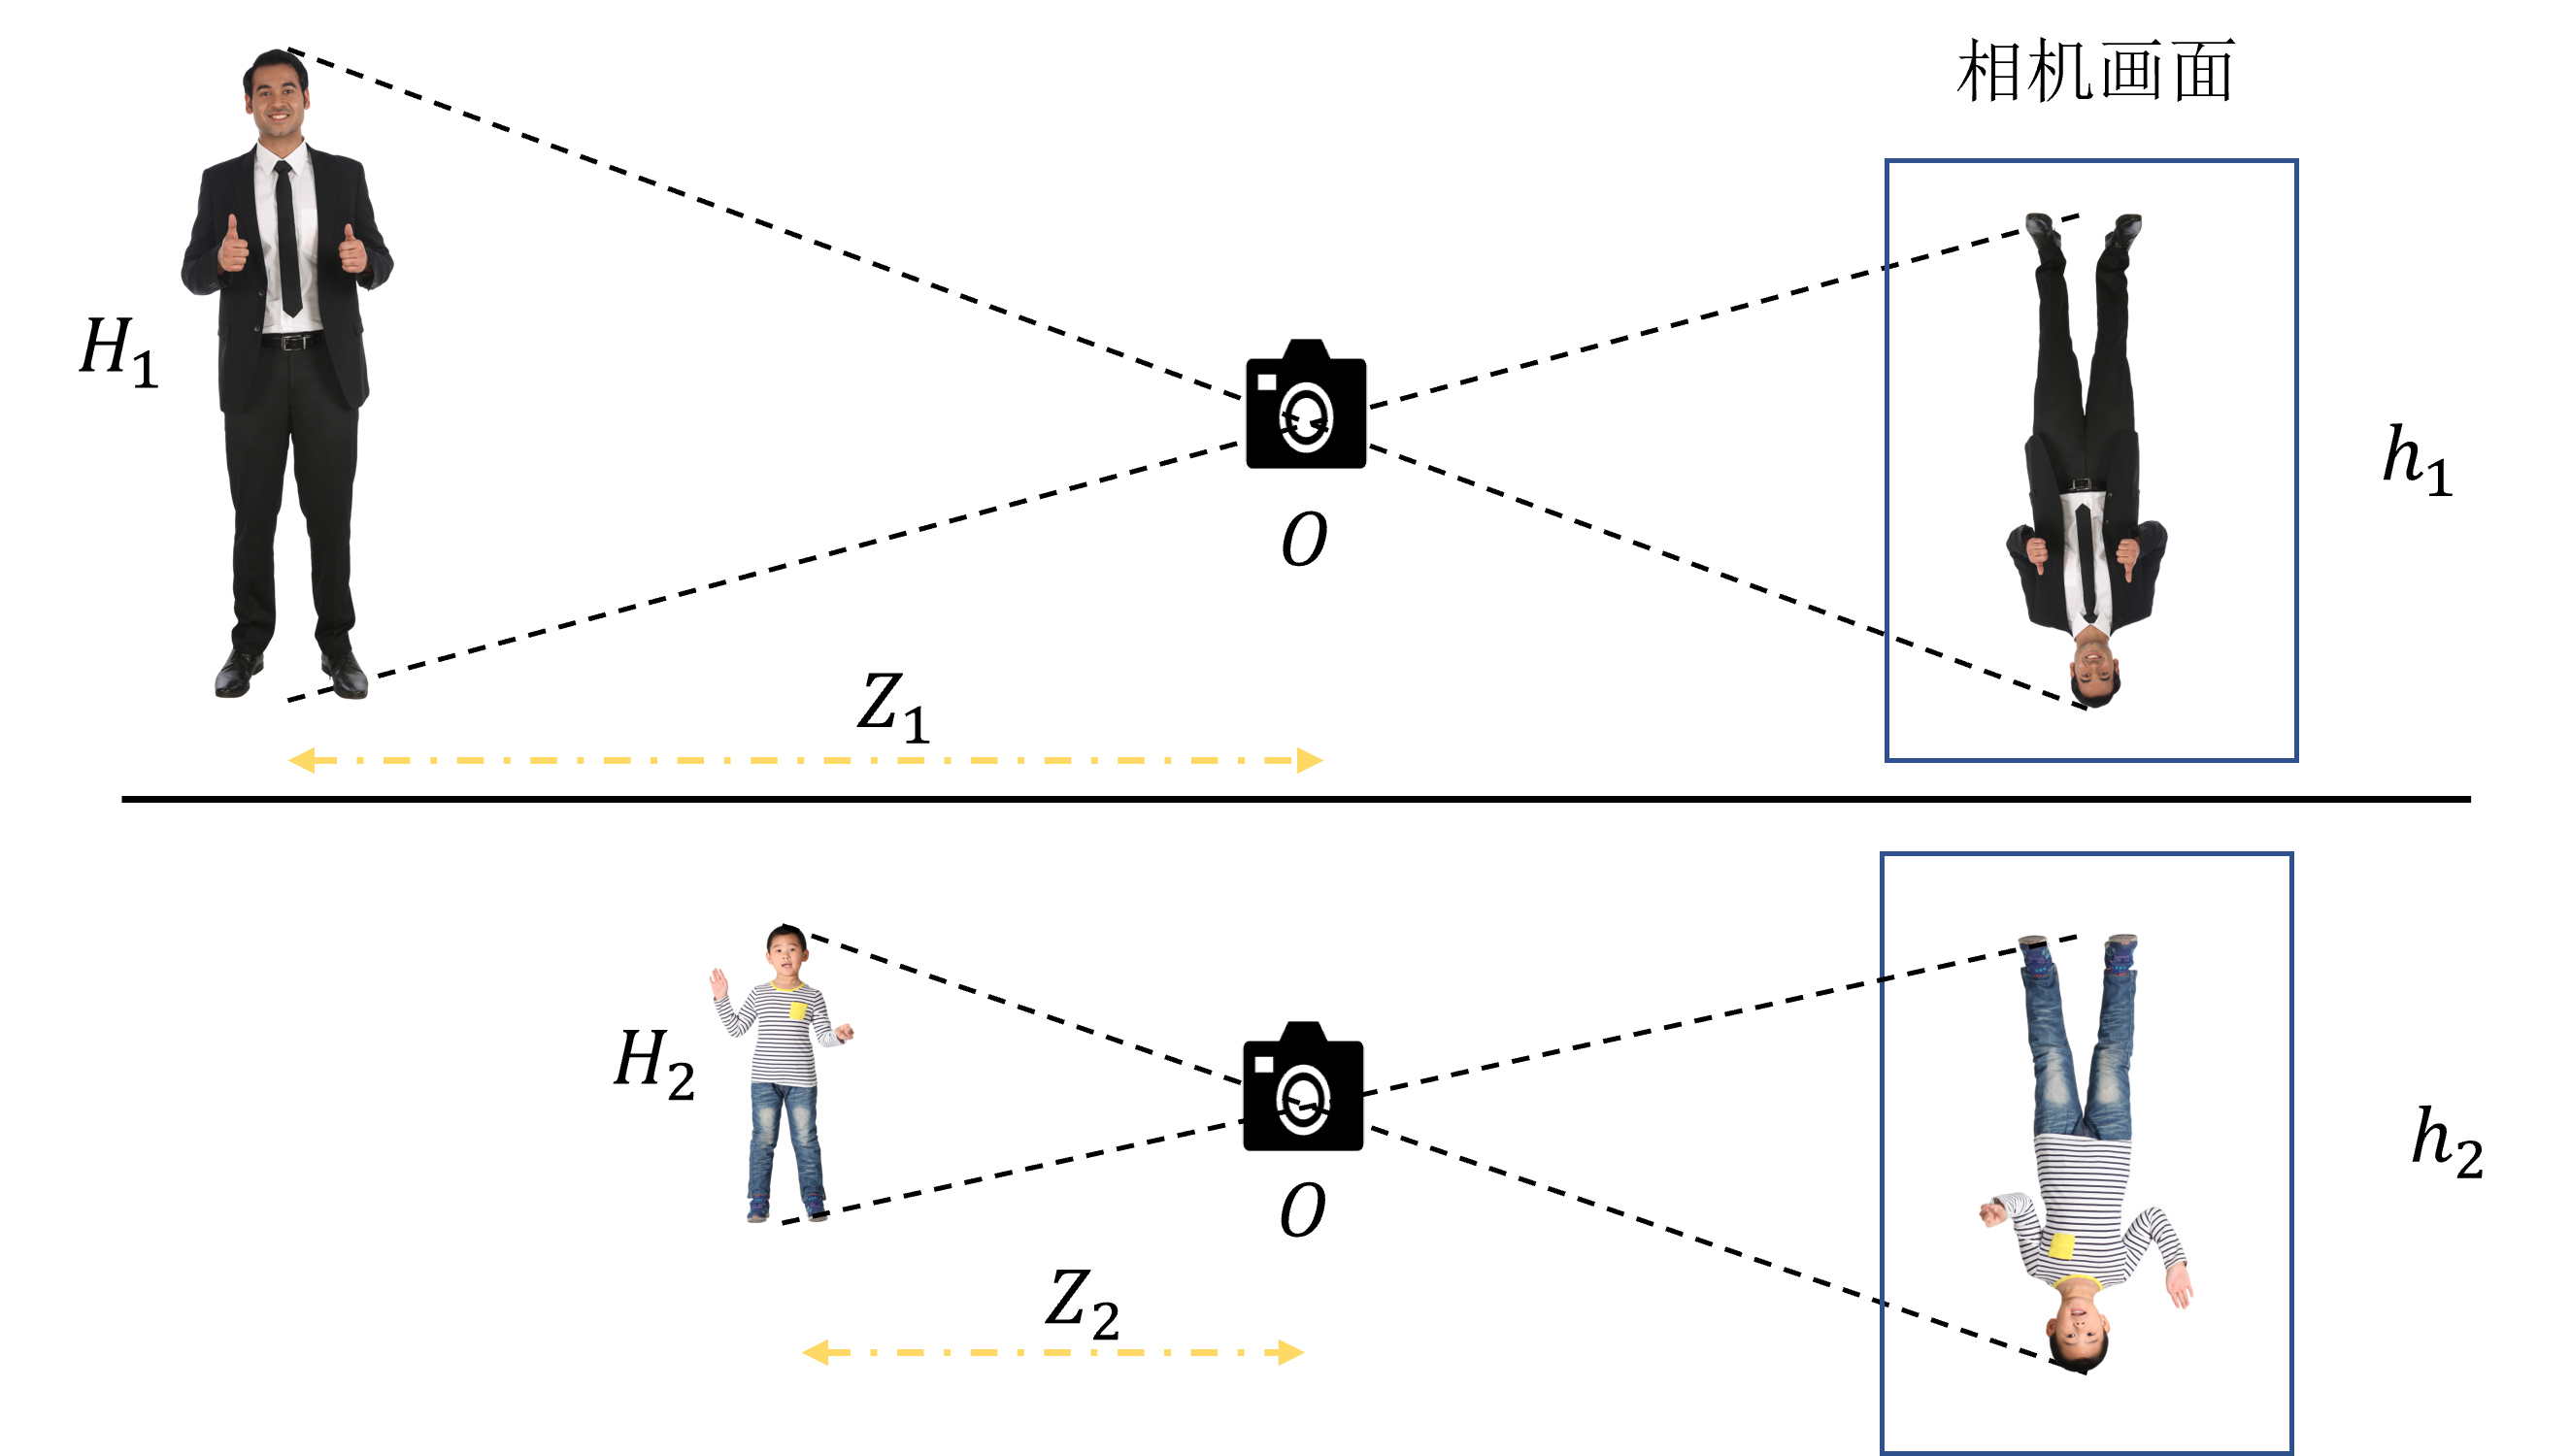
\includegraphics[width=\linewidth,height=2.6cm,keepaspectratio]{mono_scale_ambiguity.png}\\
                \scriptsize 不同三维骨架可投影为相同二维姿态，\\绝对深度无法唯一确定
            \end{block}
        \end{column}
        \begin{column}{0.48\textwidth}
            \begin{block}{\small ② 双目级联误差耦合}
                \centering
                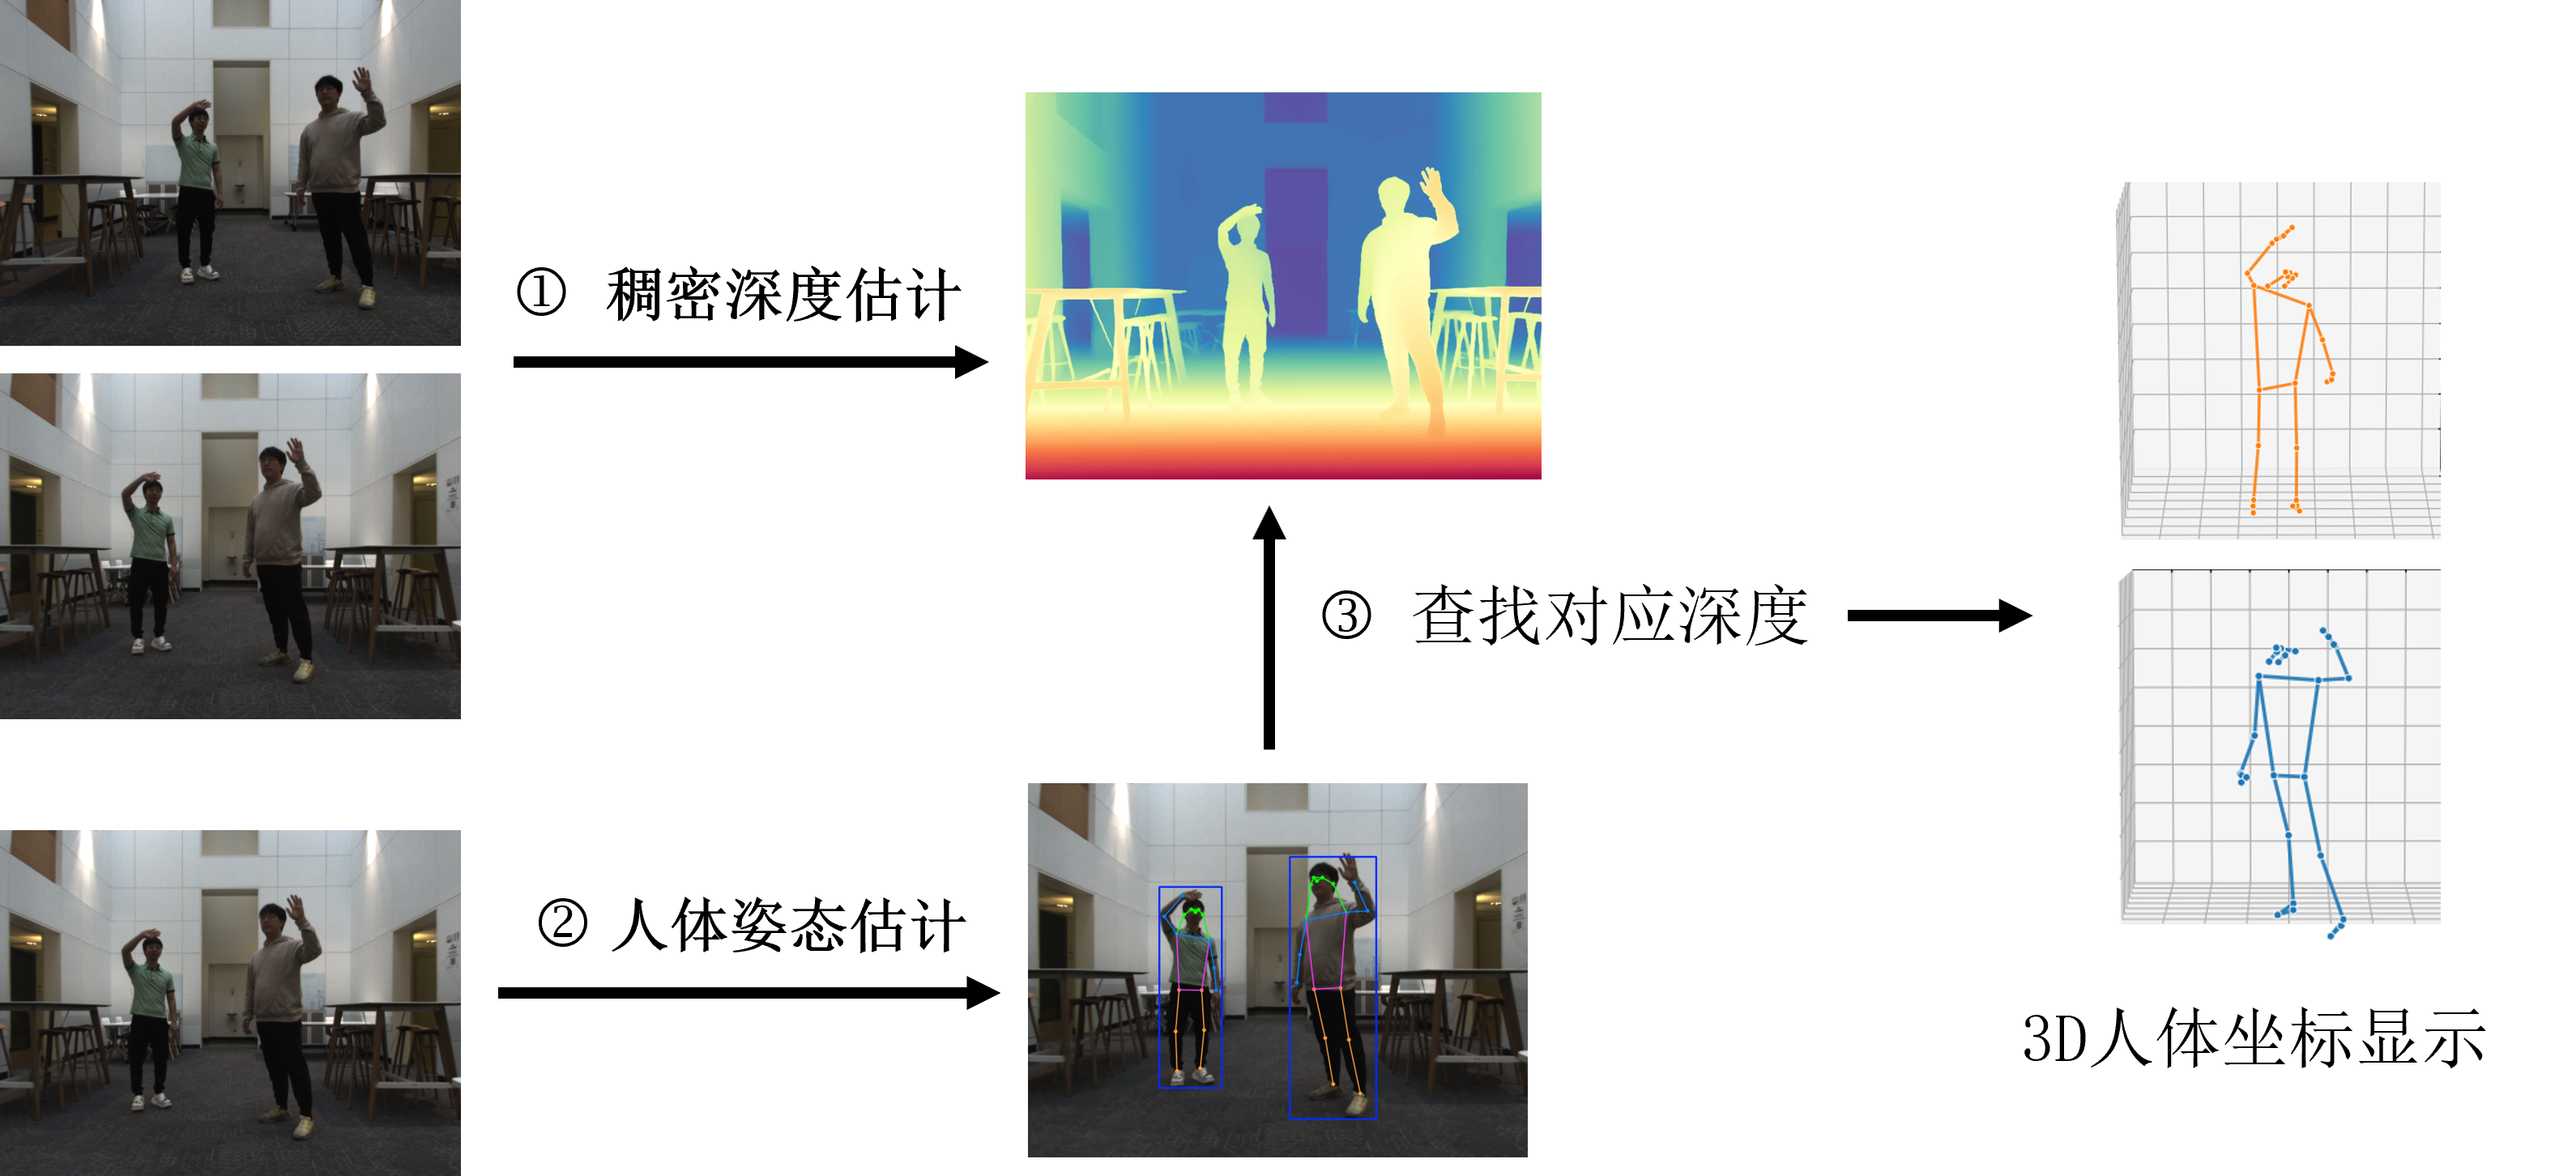
\includegraphics[width=\linewidth,height=2.6cm,keepaspectratio]{Two-Stage_Dualocular_Human_Pose_Estimation.png}\\
                \scriptsize 稠密视差图估计 + 关节点回代，\\两阶段误差逐级放大，计算冗余大
            \end{block}
        \end{column}
    \end{columns}
    \vspace{4pt}
    \begin{alertblock}{\small ③ 端侧部署：精度–速度–内存三角权衡}
        \footnotesize
        直接 INT8 全量化 → 关键层（注意力/热力图头）数值敏感，精度显著下降；\\
        保留 FP32 → 延迟/显存超预算。\textbf{需硬件感知的混合精度策略}，在有限芯片算力下找最优权衡点。
    \end{alertblock}
\end{frame}


%% ========================================
\section{相关研究}
%% ========================================

\begin{frame}{三维人体姿态估计研究现状}
    \begin{columns}
        \begin{column}{0.32\textwidth}
            \begin{block}{\centering 单目}
                \footnotesize
                HMR / SPIN / CLIFF\\
                VideoPose3D\\
                PoseFormer\\
                WHAM / NLF\\[4pt]
                \textcolor{red}{深度歧义，\\绝对尺度不稳}
            \end{block}
        \end{column}
        \begin{column}{0.32\textwidth}
            \begin{block}{\centering 多目}
                \footnotesize
                VoxelPose\\
                MVGFormer\\
                TEMPO\\
                MV-SSM\\[4pt]
                \textcolor{red}{布局固定，\\部署成本高}
            \end{block}
        \end{column}
        \begin{column}{0.32\textwidth}
            \begin{block}{\centering 双目}
                \footnotesize
                MobiDepthPose\\
                DMCPose\\
                RTMO+SGBM\\
                RTMO+MSNet\\[4pt]
                \textcolor{red}{级联误差耦合，\\端侧效率低}
            \end{block}
        \end{column}
    \end{columns}
    \vspace{8pt}
    \begin{exampleblock}{研究空白}
        \centering 面向端侧的\textbf{端到端双目三维姿态估计}与\textbf{量化部署}研究极为稀缺
    \end{exampleblock}
\end{frame}

\begin{frame}{实验数据集}
    \begin{columns}
        \begin{column}{0.52\textwidth}
            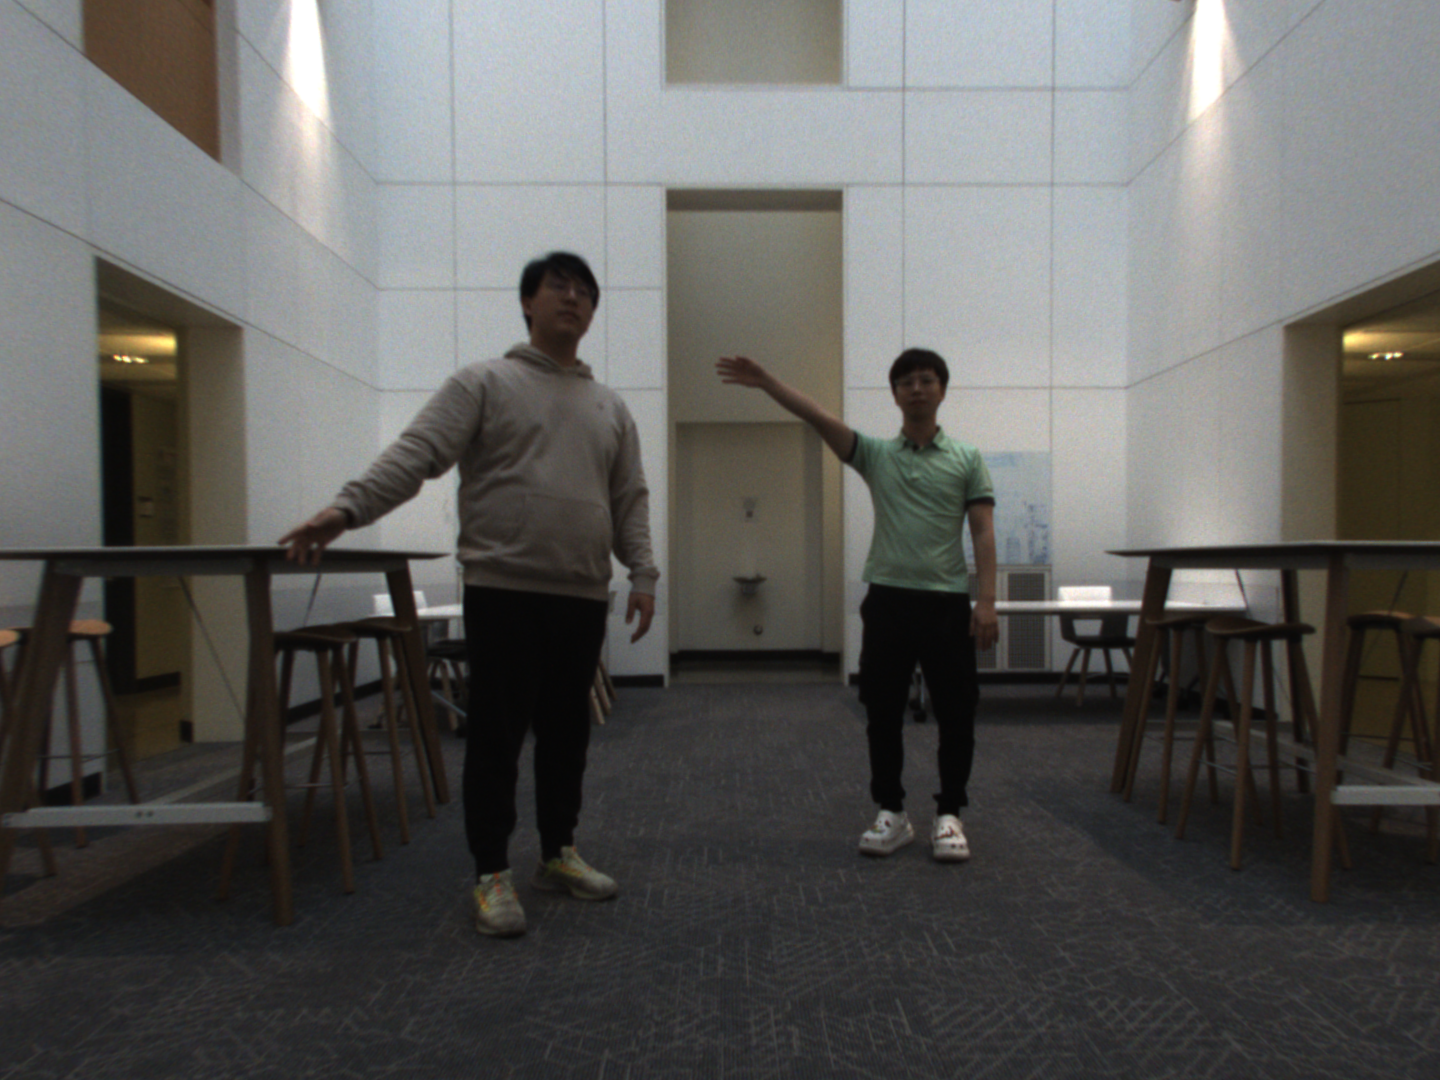
\includegraphics[width=\linewidth]{dataset.png}
        \end{column}
        \begin{column}{0.45\textwidth}
            \small
            \begin{itemize}
                \item \textbf{RT-Pose}\\
                    真实双目，室内外多场景\\多人活动、弱光、遮挡\\
                    \textcolor{deepblue}{→ 主训练/测试集}
                \vspace{6pt}
                \item \textbf{MADS}\\
                    武术/舞蹈，大幅度动作\\完整双目标定参数\\
                    \textcolor{deepblue}{→ 零样本跨域测试}
                \vspace{6pt}
                \item 评价指标：\textbf{MPJPE}（mm）
            \end{itemize}
        \end{column}
    \end{columns}
\end{frame}


%% ========================================
\section{研究方法}
%% ========================================

\begin{frame}[shrink=5]{整体框架}
    \begin{center}
        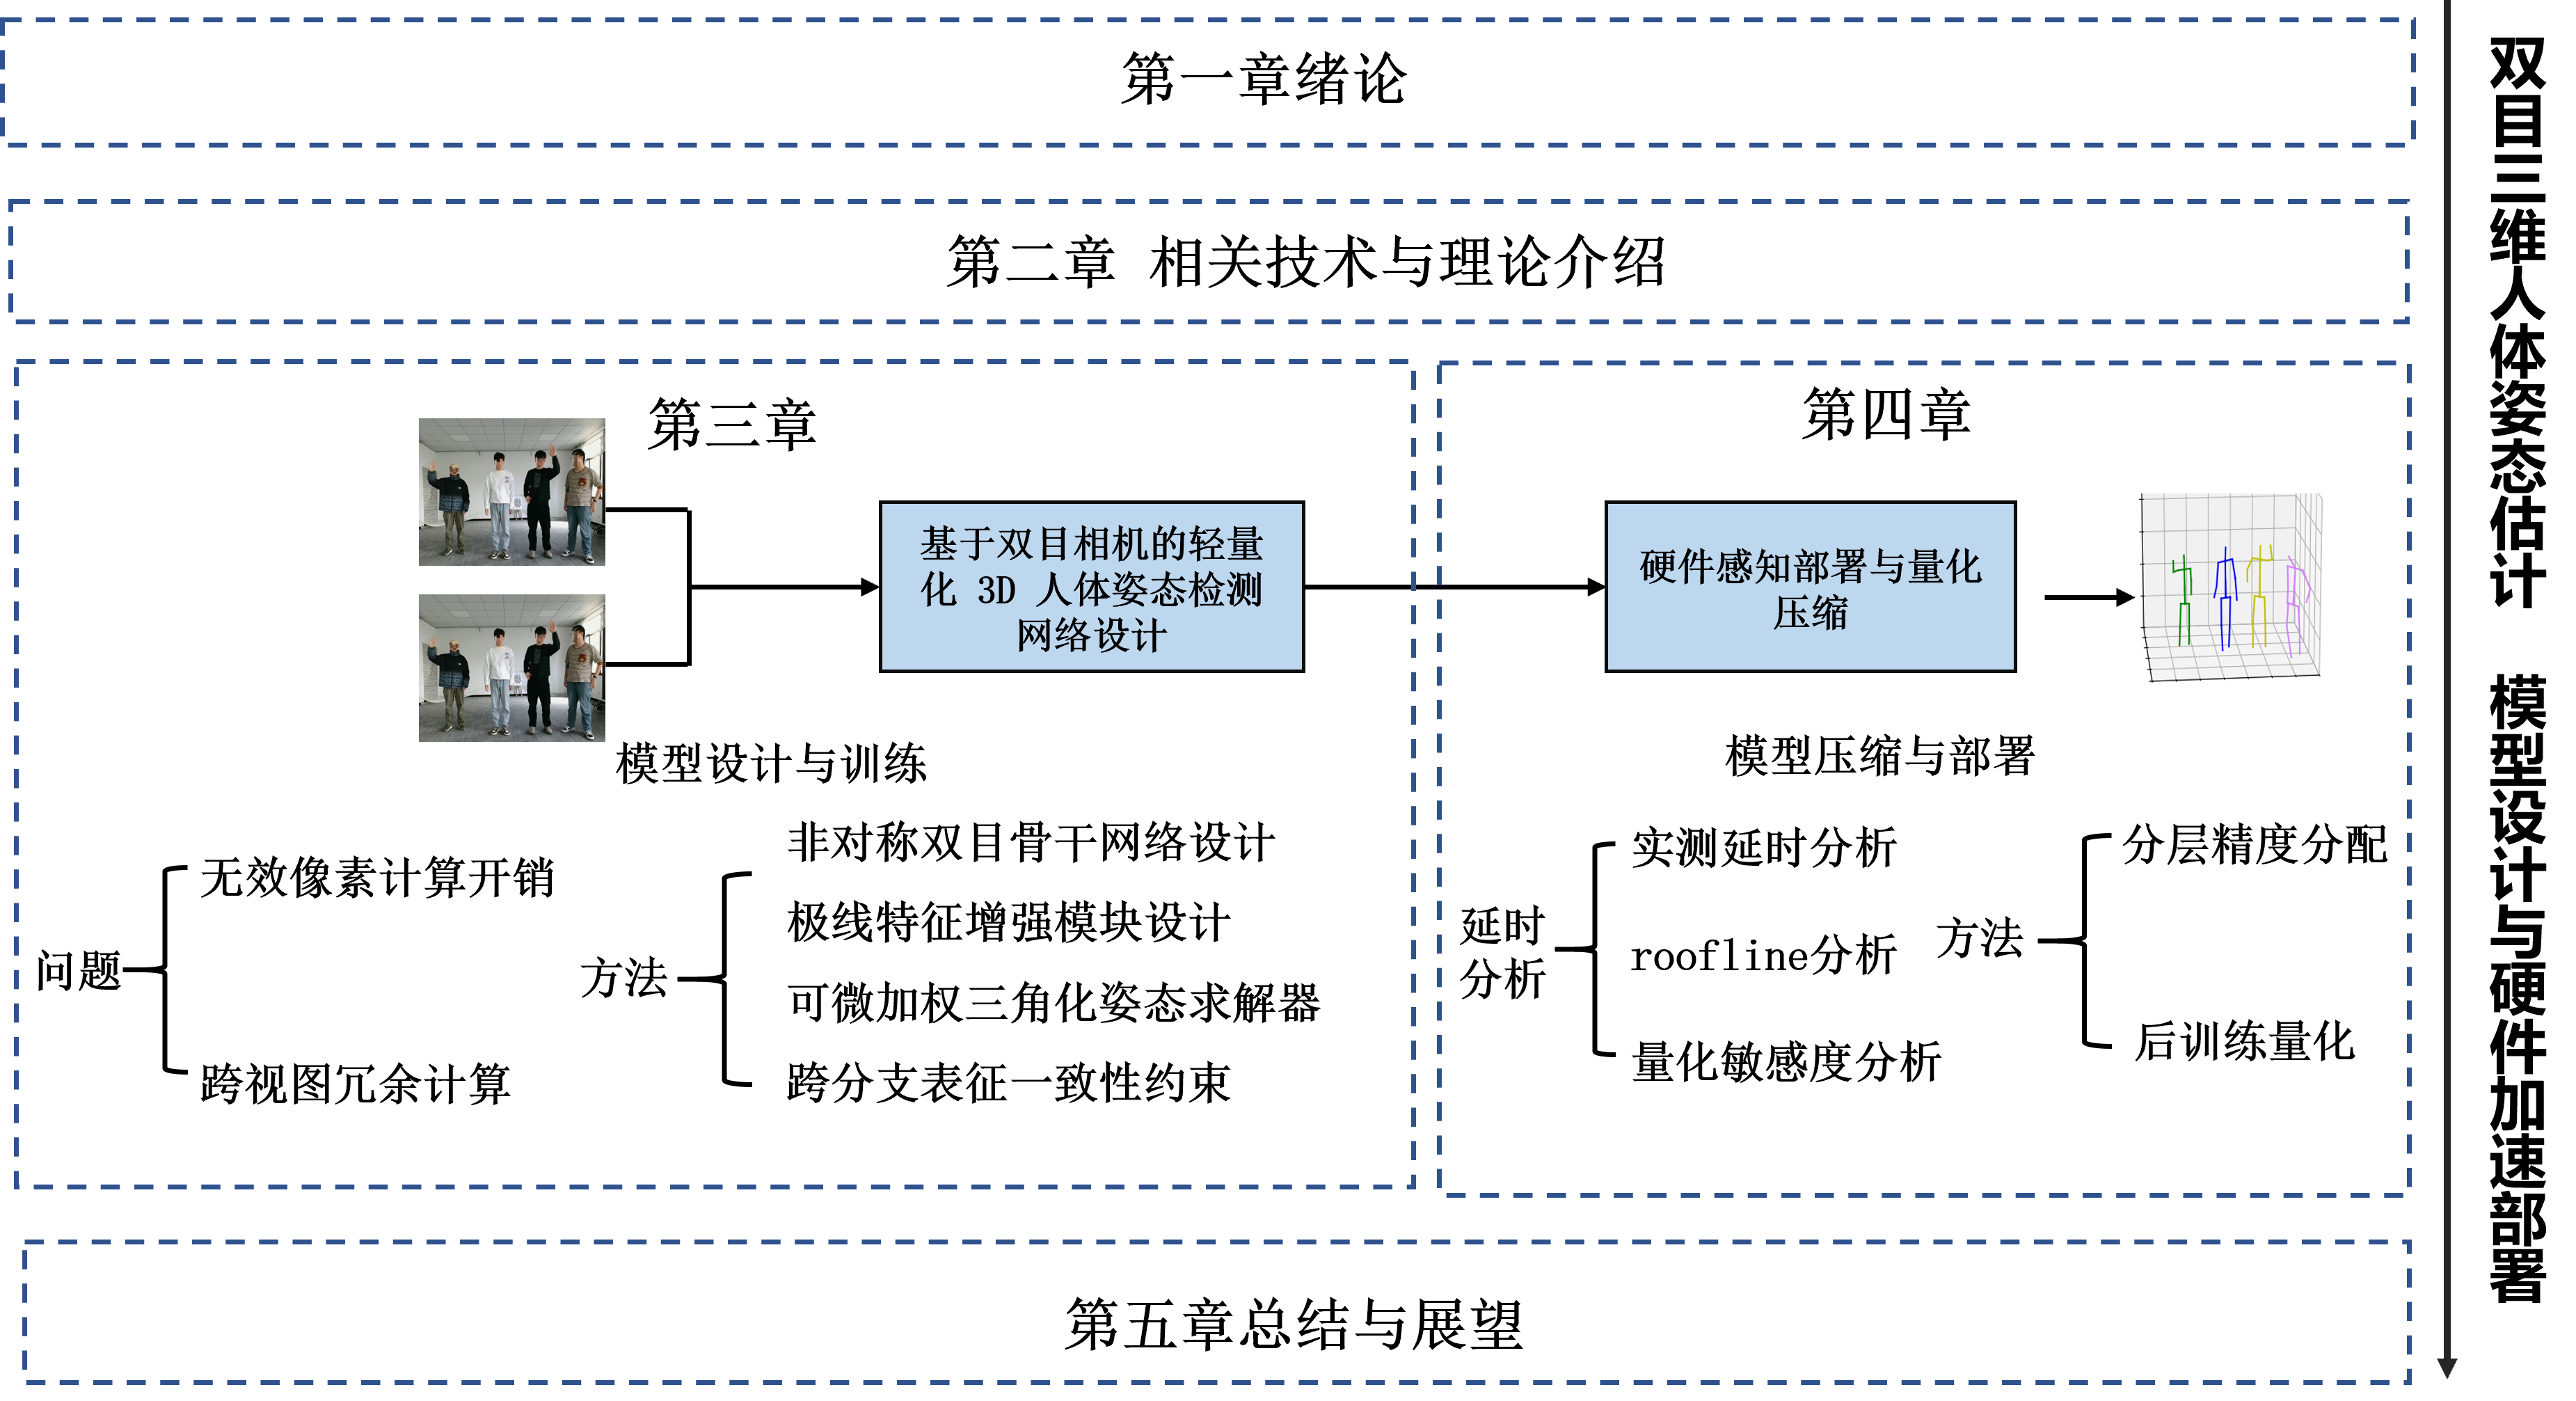
\includegraphics[width=0.95\linewidth,height=5.0cm,keepaspectratio]{OverallStructureDiagramOfTheSystem.png}
    \end{center}
    \vspace{-2pt}
    \begin{columns}
        \begin{column}{0.24\textwidth}
            \centering\footnotesize\textbf{①} 非对称双目骨干
        \end{column}
        \begin{column}{0.24\textwidth}
            \centering\footnotesize\textbf{②} 极线特征增强\\（EFEM）
        \end{column}
        \begin{column}{0.24\textwidth}
            \centering\footnotesize\textbf{③} 可微加权三角化\\（DWT）
        \end{column}
        \begin{column}{0.24\textwidth}
            \centering\footnotesize\textbf{④} 跨分支一致性\\约束（训练期）
        \end{column}
    \end{columns}
\end{frame}

\begin{frame}[shrink=3]{非对称双目骨干网络}
    \begin{columns}
        \begin{column}{0.55\textwidth}
            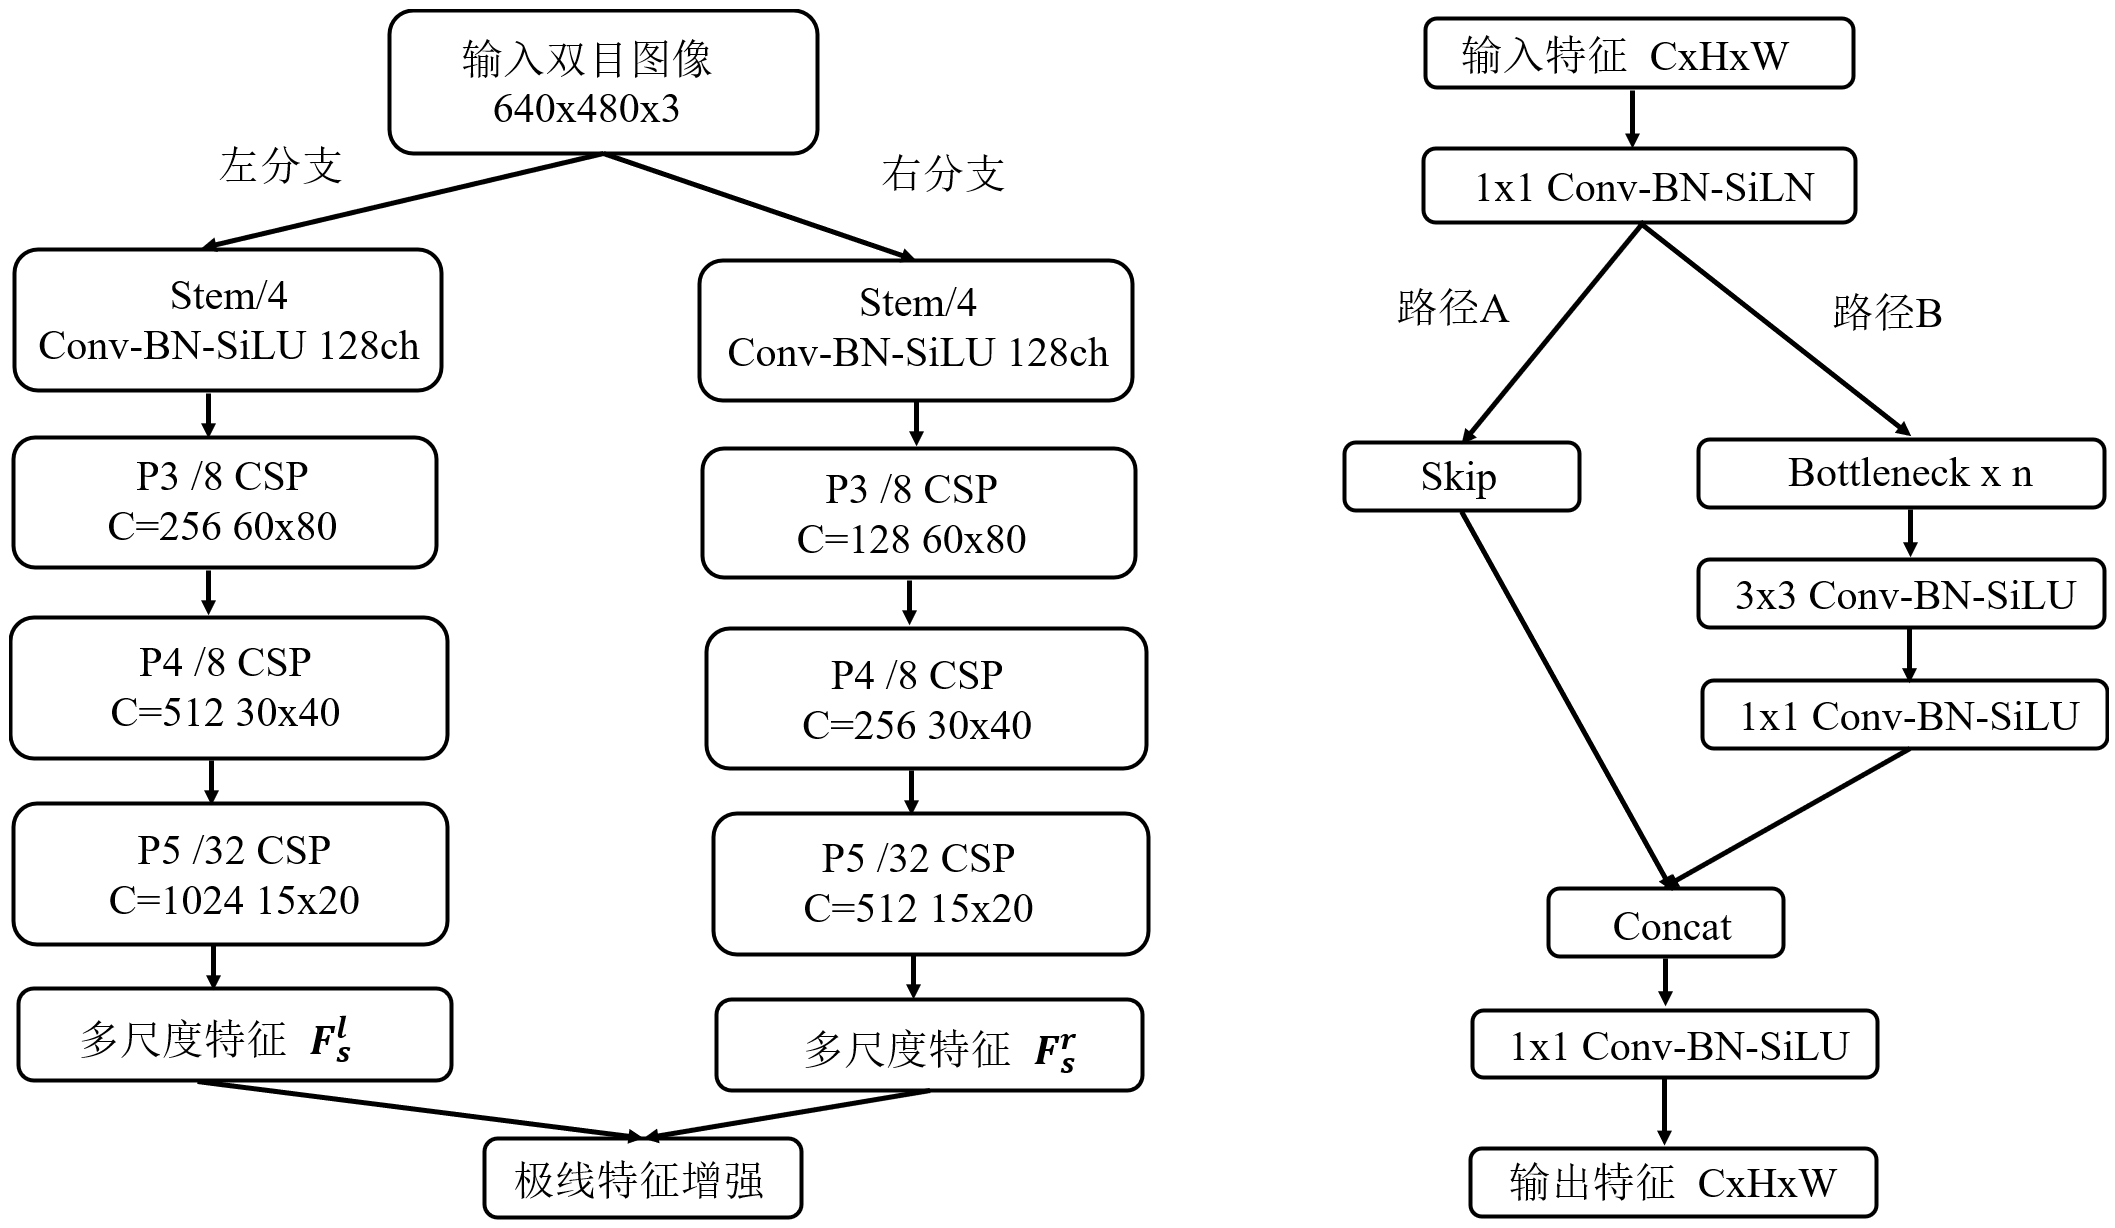
\includegraphics[width=\linewidth]{Overall_structure_of_asymmetric_binocular_backbone_network.png}
        \end{column}
        \begin{column}{0.42\textwidth}
            \small
            \begin{itemize}
                \item \textbf{问题：}对称双分支冗余大
                \item \textbf{设计：}\\
                    主视角 → 高容量骨干\\
                    辅助视角 → 轻量骨干
                \item \textbf{增强：}随机左右翻转交换，打破视角偏置
            \end{itemize}
            \vspace{6pt}
            \begin{table}
                \centering
                \footnotesize
                \begin{tabular}{lcc}
                    \toprule
                    配置 & FLOPs & MPJPE \\
                    \midrule
                    对称轻量 & 9.2G & 182.0 \\
                    对称全量 & 22.5G & 154.5 \\
                    \textbf{本文非对称} & \textbf{13.9G} & \textbf{158.6} \\
                    \bottomrule
                \end{tabular}
            \end{table}
            \footnotesize FLOPs 较对称全量↓\textbf{38\%}\\精度损失仅 4.1\,mm
        \end{column}
    \end{columns}
\end{frame}

\begin{frame}[shrink=8]{极线特征增强模块（EFEM）}
    {\centering\colorbox{white}{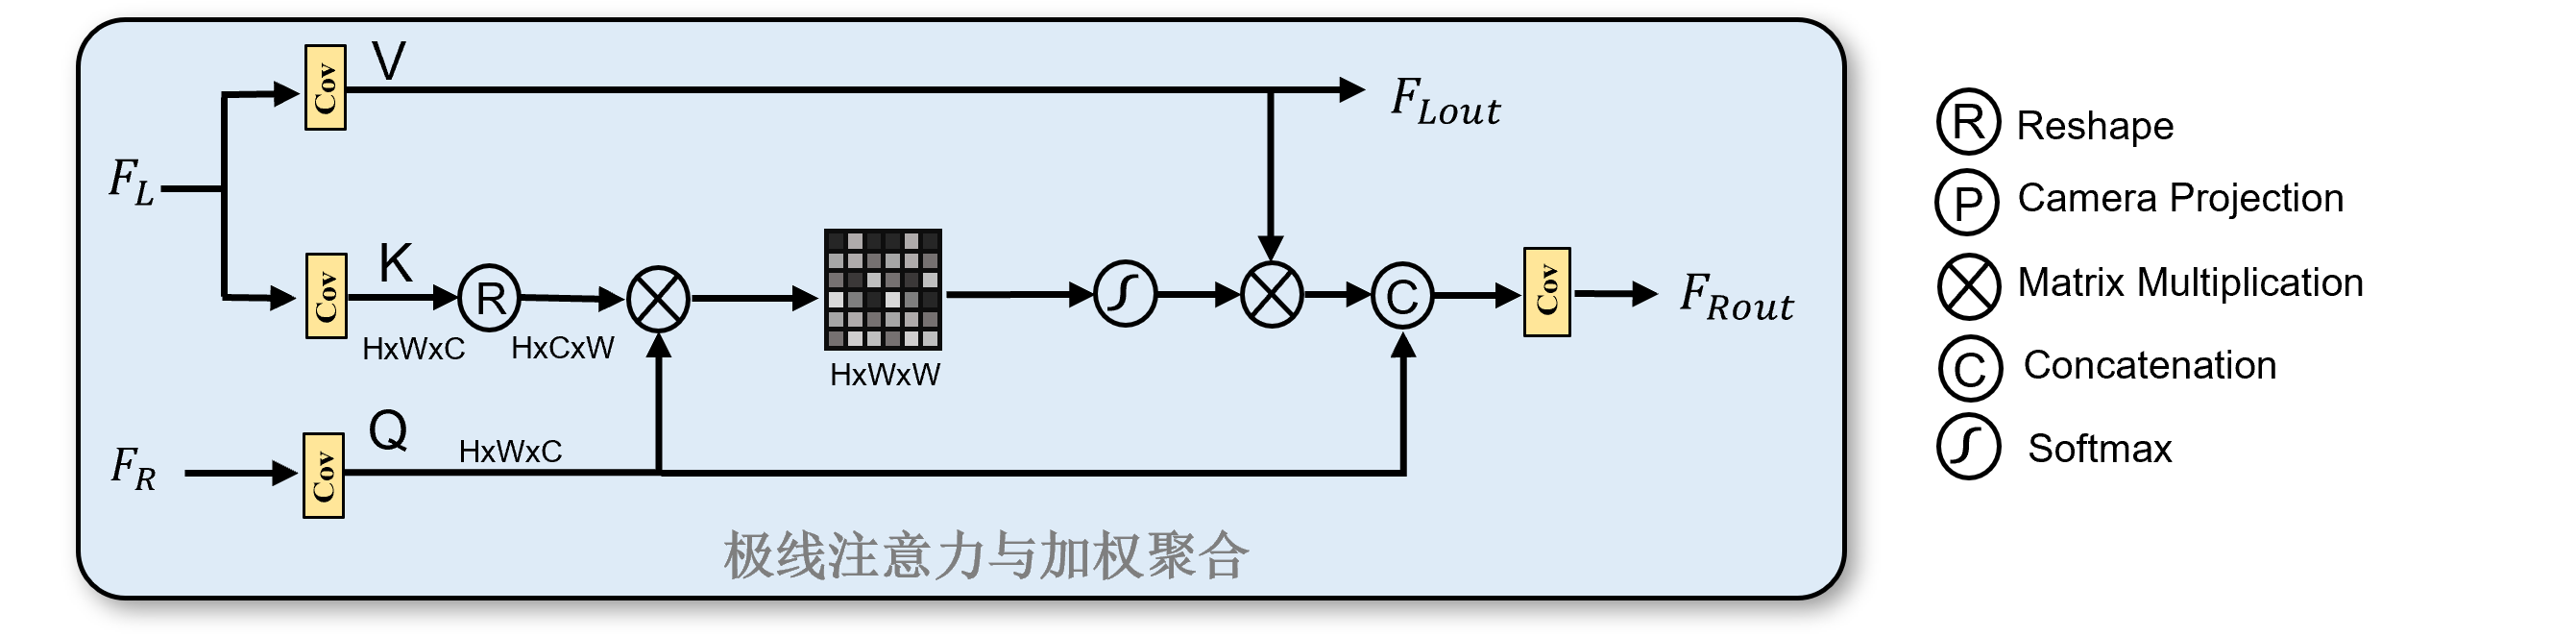
\includegraphics[width=0.95\linewidth,height=3.8cm,keepaspectratio]{Epipolar_attention_and_weighted_aggregation.png}}\\[2pt]
    \footnotesize 极线注意力采样与加权聚合示意图\par}
    \vspace{4pt}
    \begin{columns}[T]
        \begin{column}{0.56\textwidth}
            \small
            \begin{itemize}
                \item \textbf{核心思路：}将跨视图匹配限制在\textbf{一维极线搜索空间}，替代全图稠密代价体
                \item 对主视角每个位置沿极线采样候选，注意力聚合后注回主特征
                \item 搜索范围 $D_{\max}=96$，避免全图搜索的 $O(HW)$ 复杂度
            \end{itemize}
        \end{column}
        \begin{column}{0.41\textwidth}
            \begin{table}
                \centering
                \footnotesize
                \renewcommand{\arraystretch}{1.1}
                \begin{tabular}{lc}
                    \toprule
                    交互方式 & MPJPE \\
                    \midrule
                    无跨视图交互 & 374.5 \\
                    拼接+卷积 & 224.8 \\
                    \textbf{EFEM（本文）} & \textbf{158.6} \\
                    \bottomrule
                \end{tabular}
            \end{table}
            \vspace{2pt}
            \begin{exampleblock}{}
                \scriptsize EFEM 相比拼接+卷积\\精度提升 \textbf{66.2\,mm}（$\downarrow$29.4\%）
            \end{exampleblock}
        \end{column}
    \end{columns}
\end{frame}

\begin{frame}{可微加权三角化姿态求解器（DWT）}
    \begin{columns}
        \begin{column}{0.50\textwidth}
            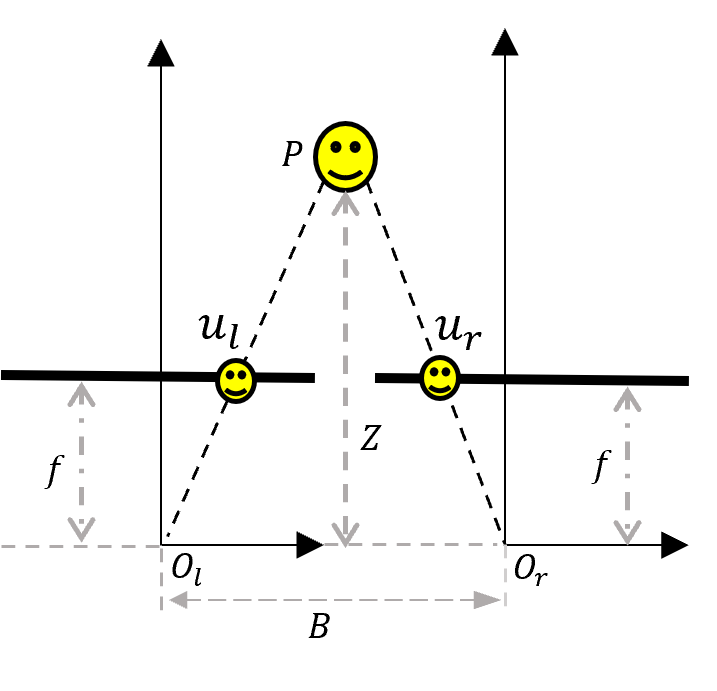
\includegraphics[width=\linewidth,height=5.5cm,keepaspectratio]{triangulation.png}
        \end{column}
        \begin{column}{0.47\textwidth}
            \footnotesize
            \textbf{三步设计：}
            \begin{enumerate}
                \item \textbf{Soft-argmax}：软期望提取二维观测，纳入反传
                $\hat{p} = \sum_{u,v}\mathrm{softmax}(\tau H)\cdot(u,v)$
                \item \textbf{置信度加权}：抑制遮挡视图干扰
                \item \textbf{显式投影约束}：最小化加权重投影误差
            \end{enumerate}
            \vspace{3pt}
            \begin{table}
                \centering
                \footnotesize
                \begin{tabular}{lc}
                    \toprule
                    三维恢复策略 & MPJPE \\
                    \midrule
                    像素级+三角化 & 277.7 \\
                    直接深度回归 & 225.1 \\
                    \textbf{DWT（本文）} & \textbf{158.6} \\
                    \bottomrule
                \end{tabular}
            \end{table}
        \end{column}
    \end{columns}
\end{frame}

\begin{frame}[shrink=3]{跨分支表征一致性约束}
    \begin{columns}[T]
        \begin{column}{0.50\textwidth}
            \begin{block}{设计思路}
                \small
                轻量辅助分支容量受限 → 几何表征不足
                \vspace{2pt}
                \begin{itemize}
                    \item 训练期：$1\!\times\!1$ 对齐卷积 + MSE 正则，引导辅助分支对齐主分支特征
                    \item \textbf{推理时完全移除}，无额外开销
                    \item 最优权重 $\lambda_{\mathrm{align}}=0.1$
                \end{itemize}
            \end{block}
            \vspace{4pt}
            \begin{exampleblock}{\small 核心模块消融（$\Delta$MPJPE，mm）}
                \scriptsize
                \setlength{\tabcolsep}{3pt}
                \renewcommand{\arraystretch}{1.0}
                \begin{tabular}{lc}
                    移除 EFEM & $+215.9$ \\
                    移除 DWT & $+119.1$ \\
                    EFEM → 拼接卷积 & $+66.2$ \\
                    对称轻量骨干 & $+23.4$ \\
                    移除一致性约束 & $+16.7$ \\
                \end{tabular}
            \end{exampleblock}
        \end{column}
        \begin{column}{0.47\textwidth}
            \vspace{2pt}
            \begin{table}
                \centering
                \small
                \caption*{一致性约束形式对比}
                \begin{tabular}{lcc}
                    \toprule
                    约束形式 & MPJPE & 提升 \\
                    \midrule
                    无约束 & 175.3 & -- \\
                    KL 散度 & 168.9 & 3.7\% \\
                    余弦相似度 & 165.2 & 5.8\% \\
                    \textbf{卷积+MSE} & \textbf{158.6} & \textbf{9.5\%} \\
                    \bottomrule
                \end{tabular}
            \end{table}
        \end{column}
    \end{columns}
\end{frame}


%% ========================================
\section{实验结果}
%% ========================================

\begin{frame}{RT-Pose 数据集对比实验}
    \begin{table}
        \centering
        \footnotesize
        \renewcommand{\arraystretch}{1.1}
        \begin{tabular}{lccc}
            \toprule
            方法 & MPJPE (mm)$\downarrow$ & 参数量 (M) & FLOPs (G) \\
            \midrule
            \multicolumn{4}{l}{\textit{单目方法（仅左视图）}} \\
            Simple Baseline & 374.3 & 23.48 & 67.19 \\
            JointFormer & 337.2 & 48.61 & 160.66 \\
            RTMW3D & 307.3 & 92.30 & 136.56 \\
            \midrule
            \multicolumn{4}{l}{\textit{双目方法（级联范式）}} \\
            MobiDepthPose & 215.3 & 7.27 & 10.36 \\
            DMCPose & 196.8 & 27.10 & 41.10 \\
            RTMO+SGBM & 211.9 & 9.80 & 12.13 \\
            RTMO+MobileStereoNet & 202.0 & 12.09 & 116.12 \\
            \midrule
            \textbf{本文方法} & \textbf{158.6} & \textbf{11.70} & \textbf{13.93} \\
            \bottomrule
        \end{tabular}
    \end{table}
    \vspace{2pt}
    \footnotesize\centering
    较最优单目 RTMW3D 降低 \textbf{148.7\,mm}；较最优双目 DMCPose 降低 \textbf{38.2\,mm}；FLOPs 仅为 RTMO+MSNet 的 \textbf{12\%}
\end{frame}

\begin{frame}[shrink=3]{定性结果 \& 零样本泛化}
    \begin{columns}[T]
        \begin{column}{0.54\textwidth}
            {\centering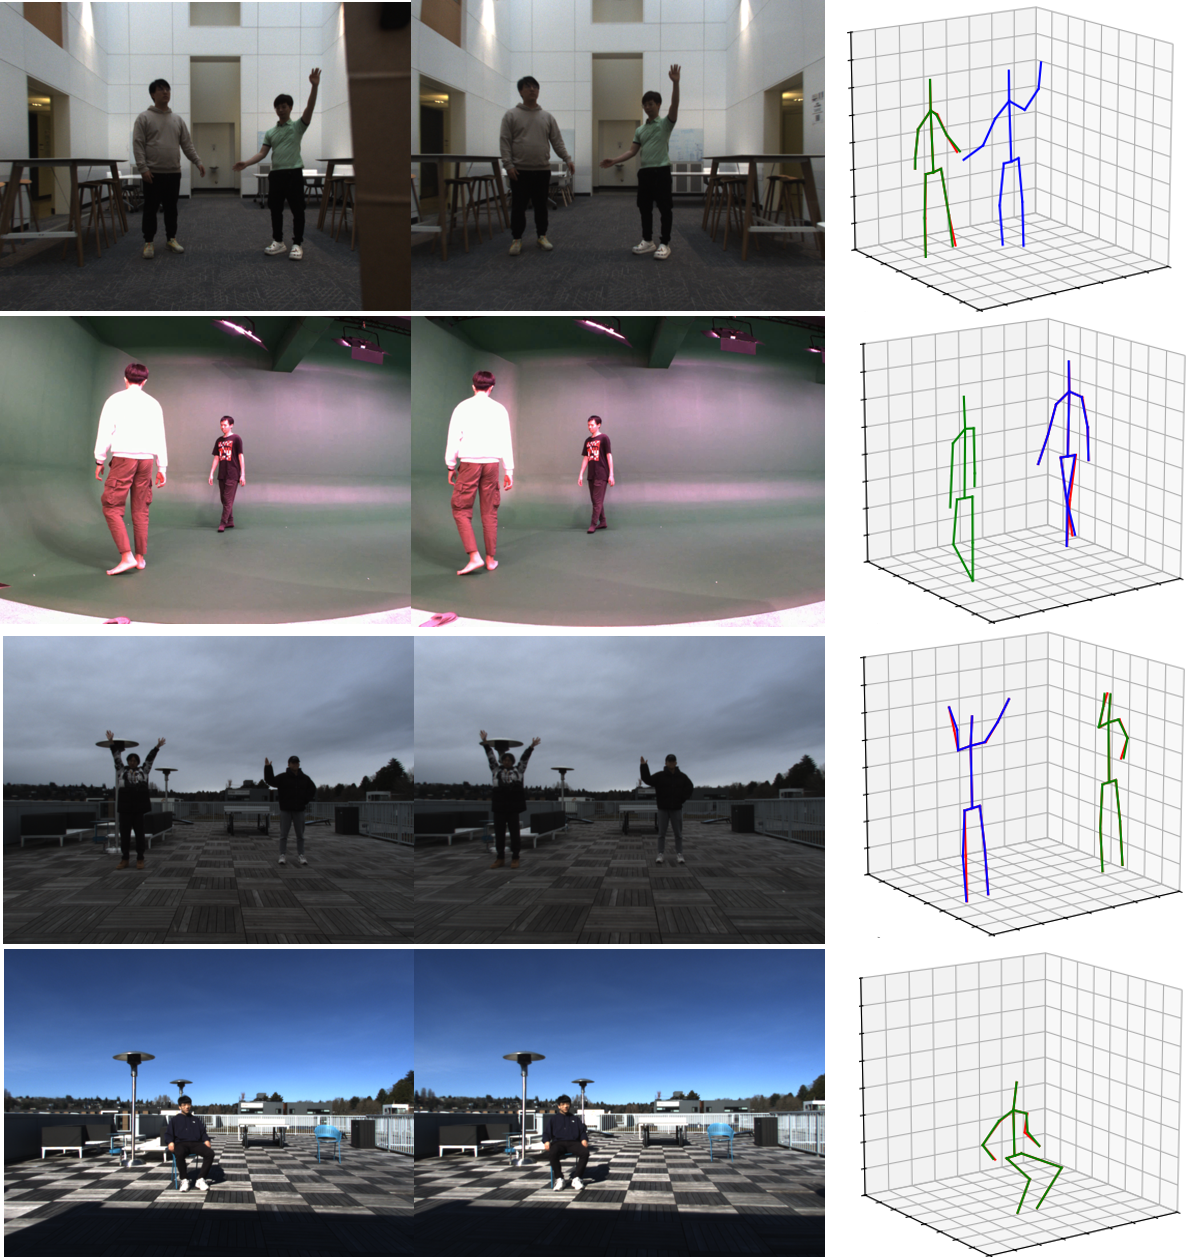
\includegraphics[width=\linewidth,height=5.0cm,keepaspectratio]{rtpose_qualitative.png}\\[2pt]
            \footnotesize RT-Pose 多人遮挡场景定性结果\par}
        \end{column}
        \begin{column}{0.43\textwidth}
            \scriptsize\textbf{RT-Pose $\to$ MADS 零样本（不微调）}
            \vspace{1pt}
            \begin{table}
                \centering
                \scriptsize
                \renewcommand{\arraystretch}{1.0}
                \begin{tabular}{lc}
                    \toprule
                    方法 & MPJPE (mm) \\
                    \midrule
                    RTMW3D & 69.6 \\
                    RTMO+SGBM & 58.0 \\
                    RTMO+MSNet & 51.2 \\
                    \textbf{本文} & \textbf{33.68} \\
                    \bottomrule
                \end{tabular}
            \end{table}
            \vspace{3pt}
            \scriptsize\textbf{多人场景时延（ms，Xiaomi 14）}
            \vspace{1pt}
            \begin{table}
                \centering
                \scriptsize
                \setlength{\tabcolsep}{3pt}
                \renewcommand{\arraystretch}{1.0}
                \begin{tabular}{lccc}
                    \toprule
                    & 1人 & 5人 & 10人 \\
                    \midrule
                    \textbf{本文} & \textbf{116.0} & \textbf{116.9} & \textbf{117.3} \\
                    RTMW3D & 436.5 & 1236.8 & 2396.4 \\
                    \bottomrule
                \end{tabular}
            \end{table}
            \vspace{3pt}
            \begin{exampleblock}{}
                \scriptsize 跨域零样本优于全部对比方法；1\textasciitilde10人时延近乎恒定
            \end{exampleblock}
        \end{column}
    \end{columns}
\end{frame}

%% ---- 量化 slide 1/4 ----
\begin{frame}{端侧推理瓶颈分析}
    \begin{columns}[T]
        \begin{column}{0.48\textwidth}
            {\centering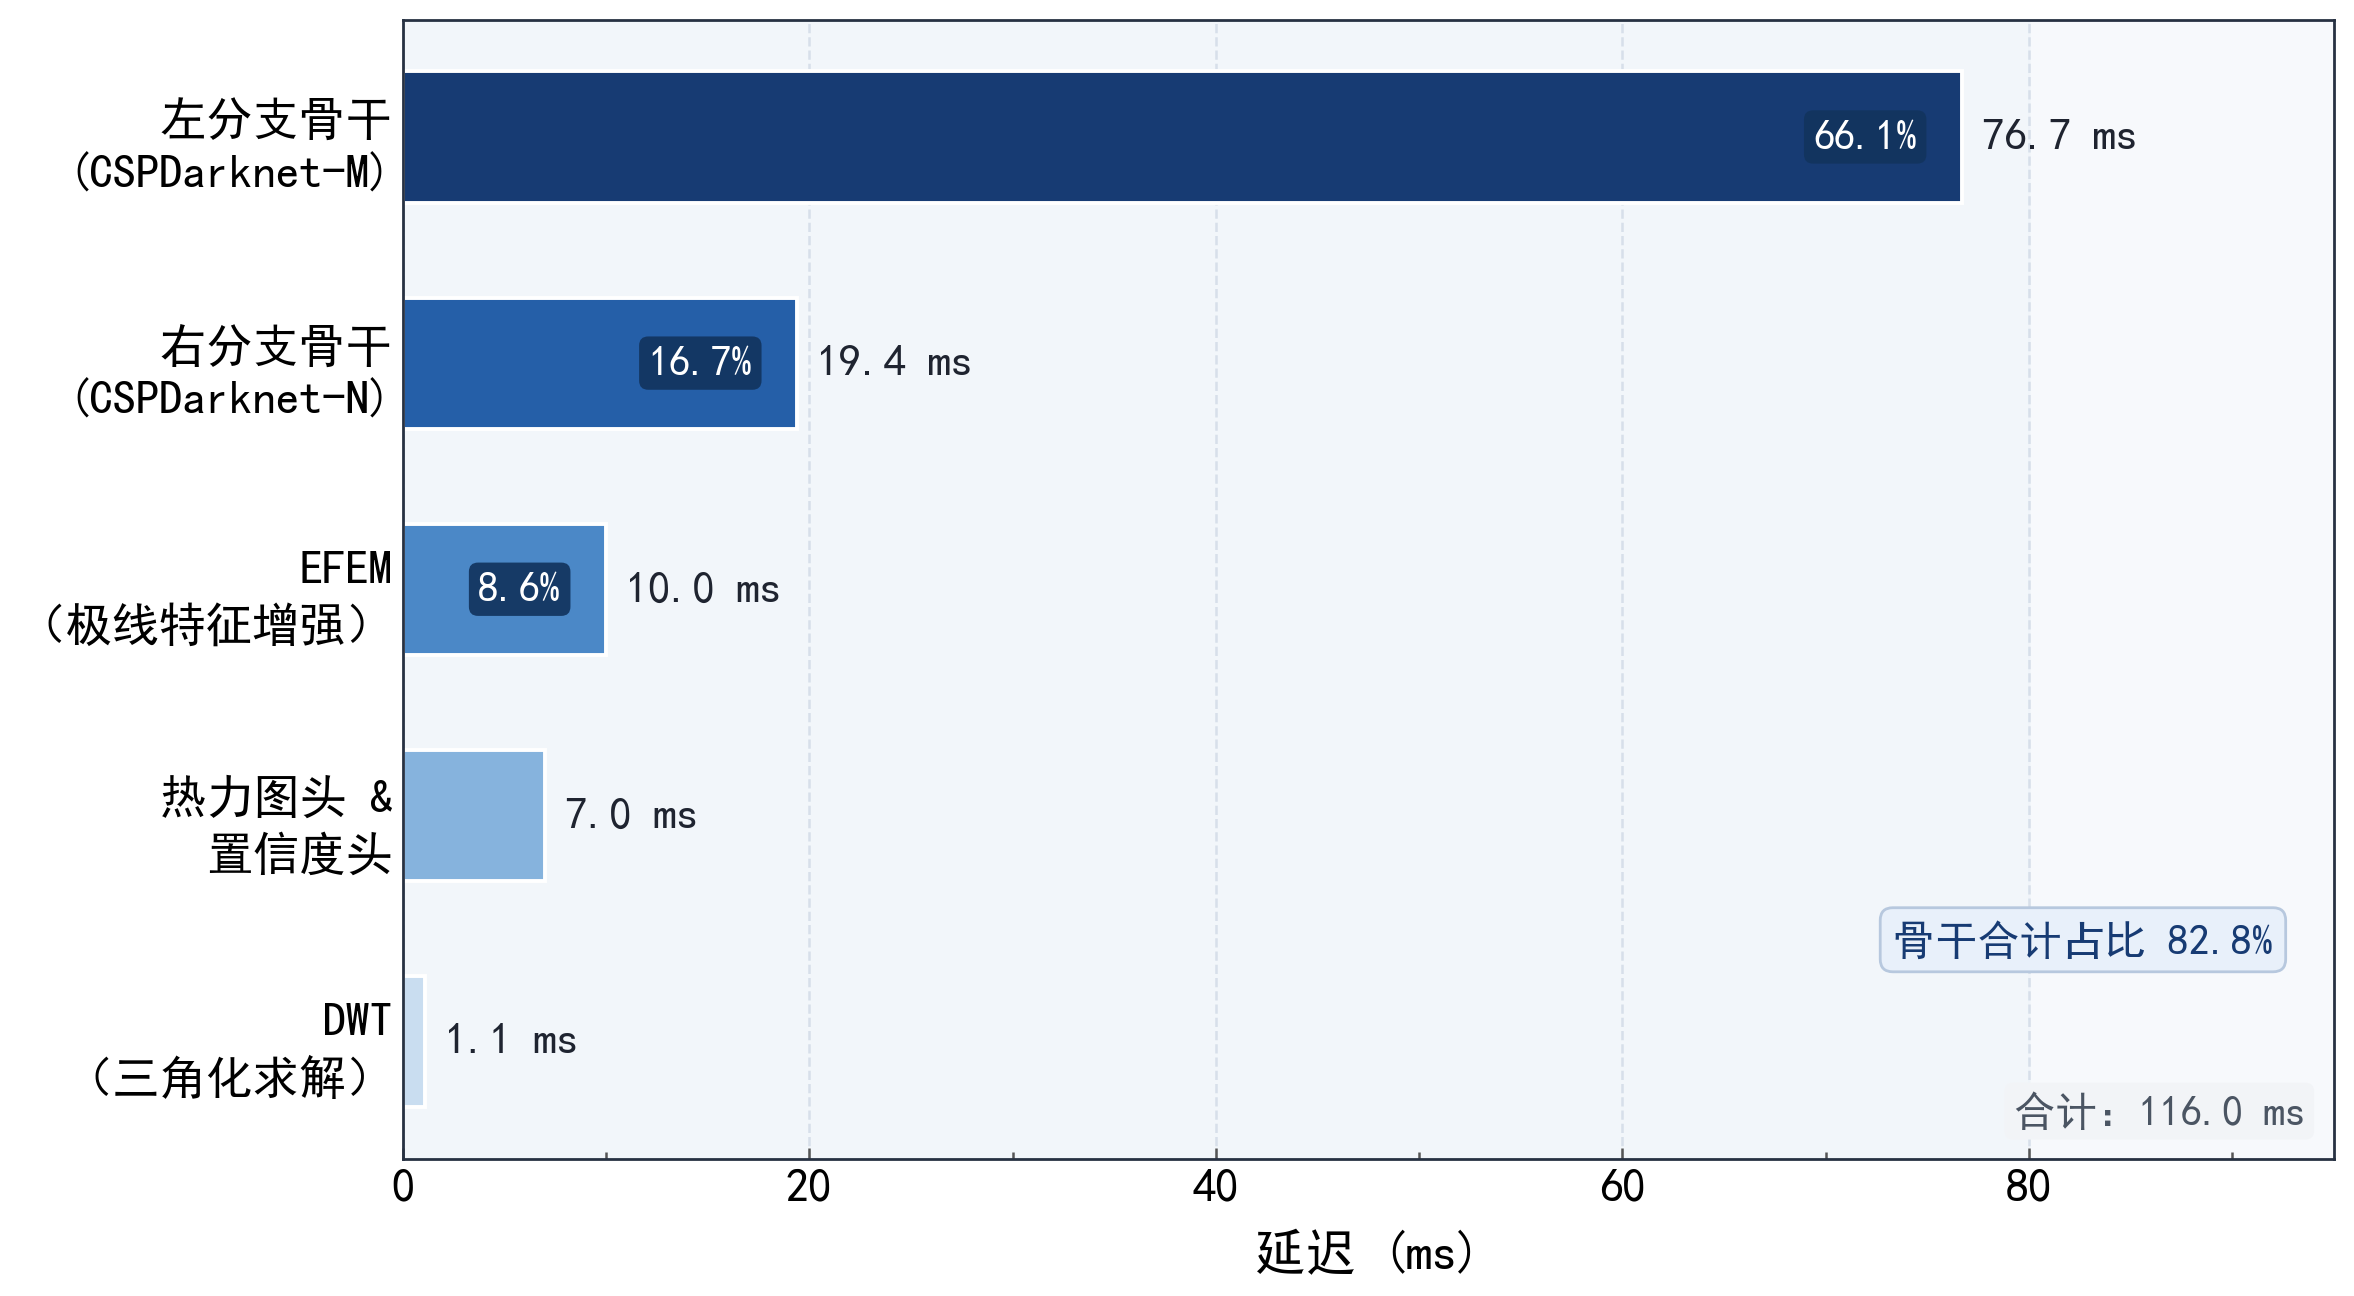
\includegraphics[width=0.9\linewidth,height=3.2cm,keepaspectratio]{ModuleDelayRatioFanChart.png}\\[1pt]
            \scriptsize 各模块端到端延迟占比\par}
            \vspace{1pt}
            \begin{table}
                \centering
                \scriptsize
                \setlength{\tabcolsep}{3pt}
                \renewcommand{\arraystretch}{1.05}
                \begin{tabular}{lcc}
                    \toprule
                    模块 & 延迟(ms) & 占比 \\
                    \midrule
                    主骨干（左视角） & 76.7 & 66.1\% \\
                    辅助骨干（右视角） & 19.4 & 16.7\% \\
                    EFEM & 10.0 & 8.6\% \\
                    热力图/置信头 & 7.0 & 6.0\% \\
                    DWT & 1.1 & 0.9\% \\
                    \midrule
                    总计 & 116.0 & 100\% \\
                    \bottomrule
                \end{tabular}
            \end{table}
        \end{column}
        \begin{column}{0.48\textwidth}
            {\centering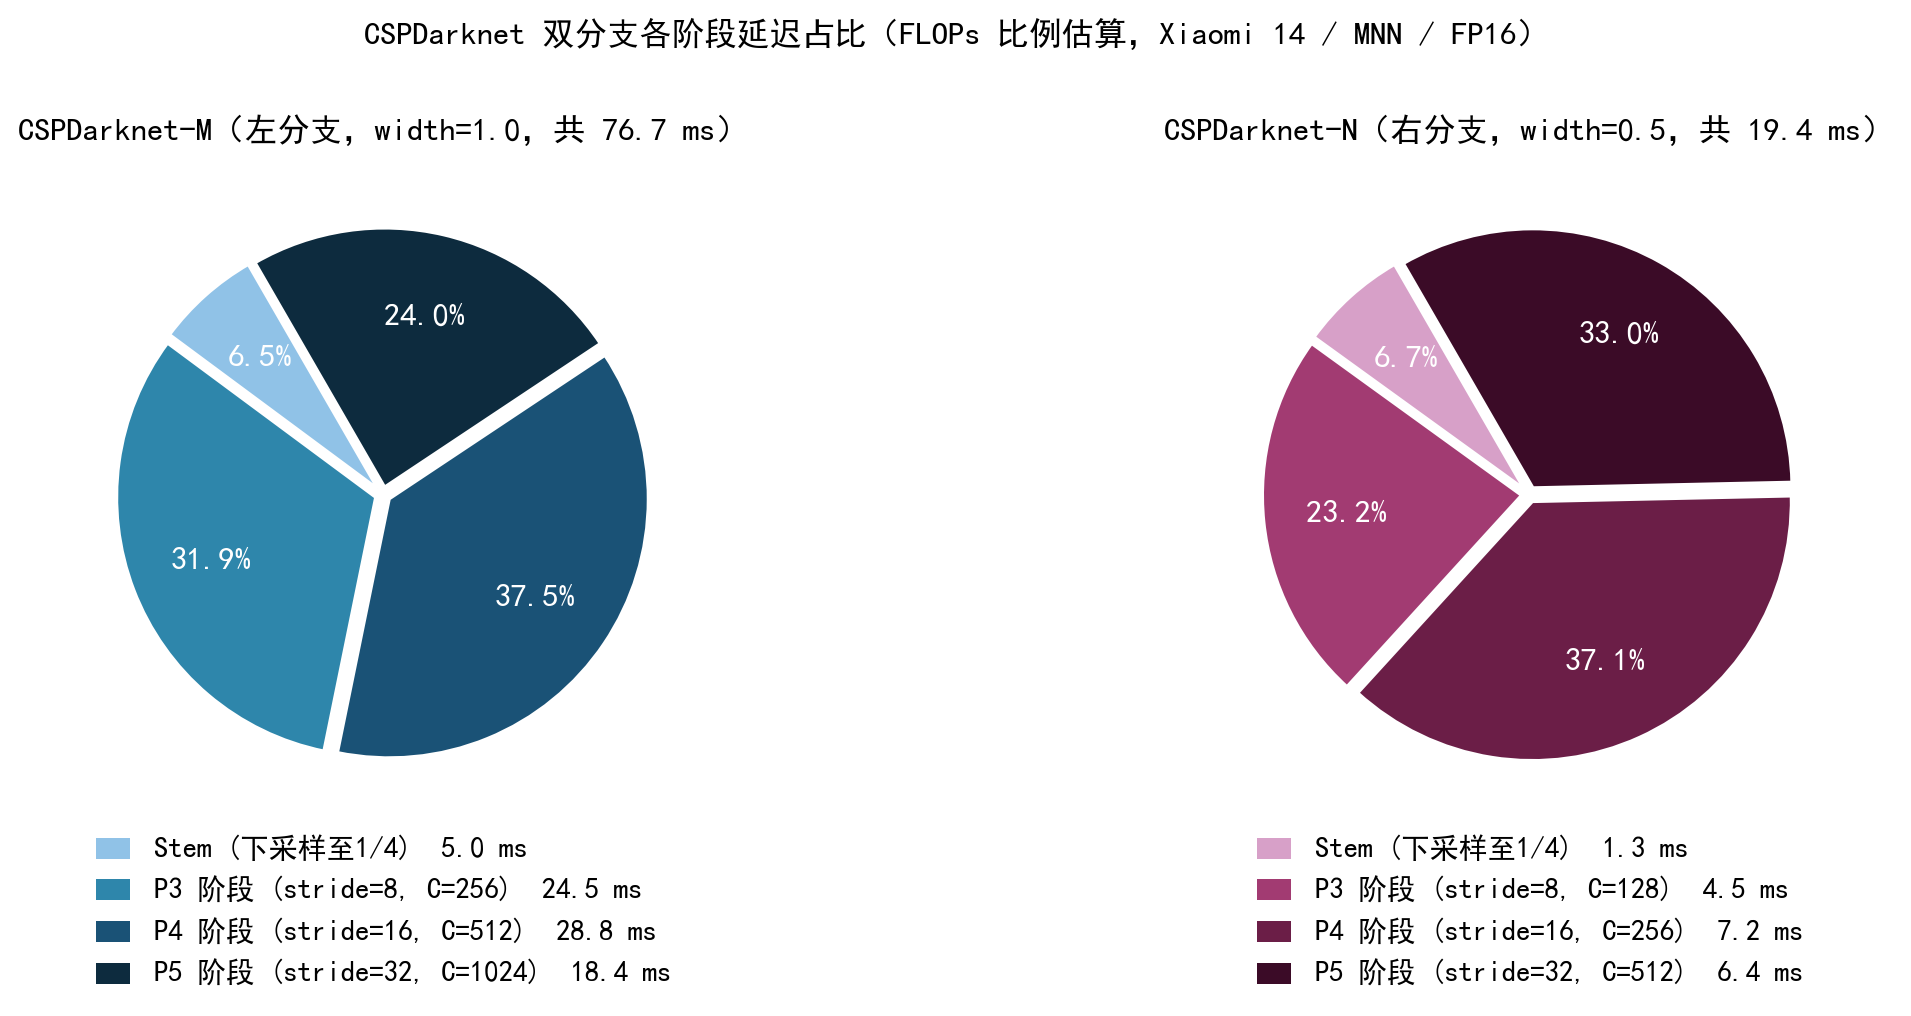
\includegraphics[width=0.9\linewidth,height=3.2cm,keepaspectratio]{CSPDarknetStageLatencyPie.png}\\[1pt]
            \scriptsize CSPDarknet 各阶段延迟分布\par}
            \vspace{1pt}
            \begin{exampleblock}{\small 分析结论}
                \scriptsize
                \begin{itemize}
                    \item 骨干卷积占总延迟 \textbf{82.8\%}，是优化首要目标
                    \item EFEM gather/correlation：极度内存密集型，量化收益有限
                    \item 热力图头、DWT：精度敏感，量化风险高
                \end{itemize}
            \end{exampleblock}
        \end{column}
    \end{columns}
\end{frame}

%% ---- 量化 slide 2/4 ----
\begin{frame}[shrink=8]{Roofline 分析与量化敏感性}
    \begin{columns}[T]
        \begin{column}{0.50\textwidth}
            {\centering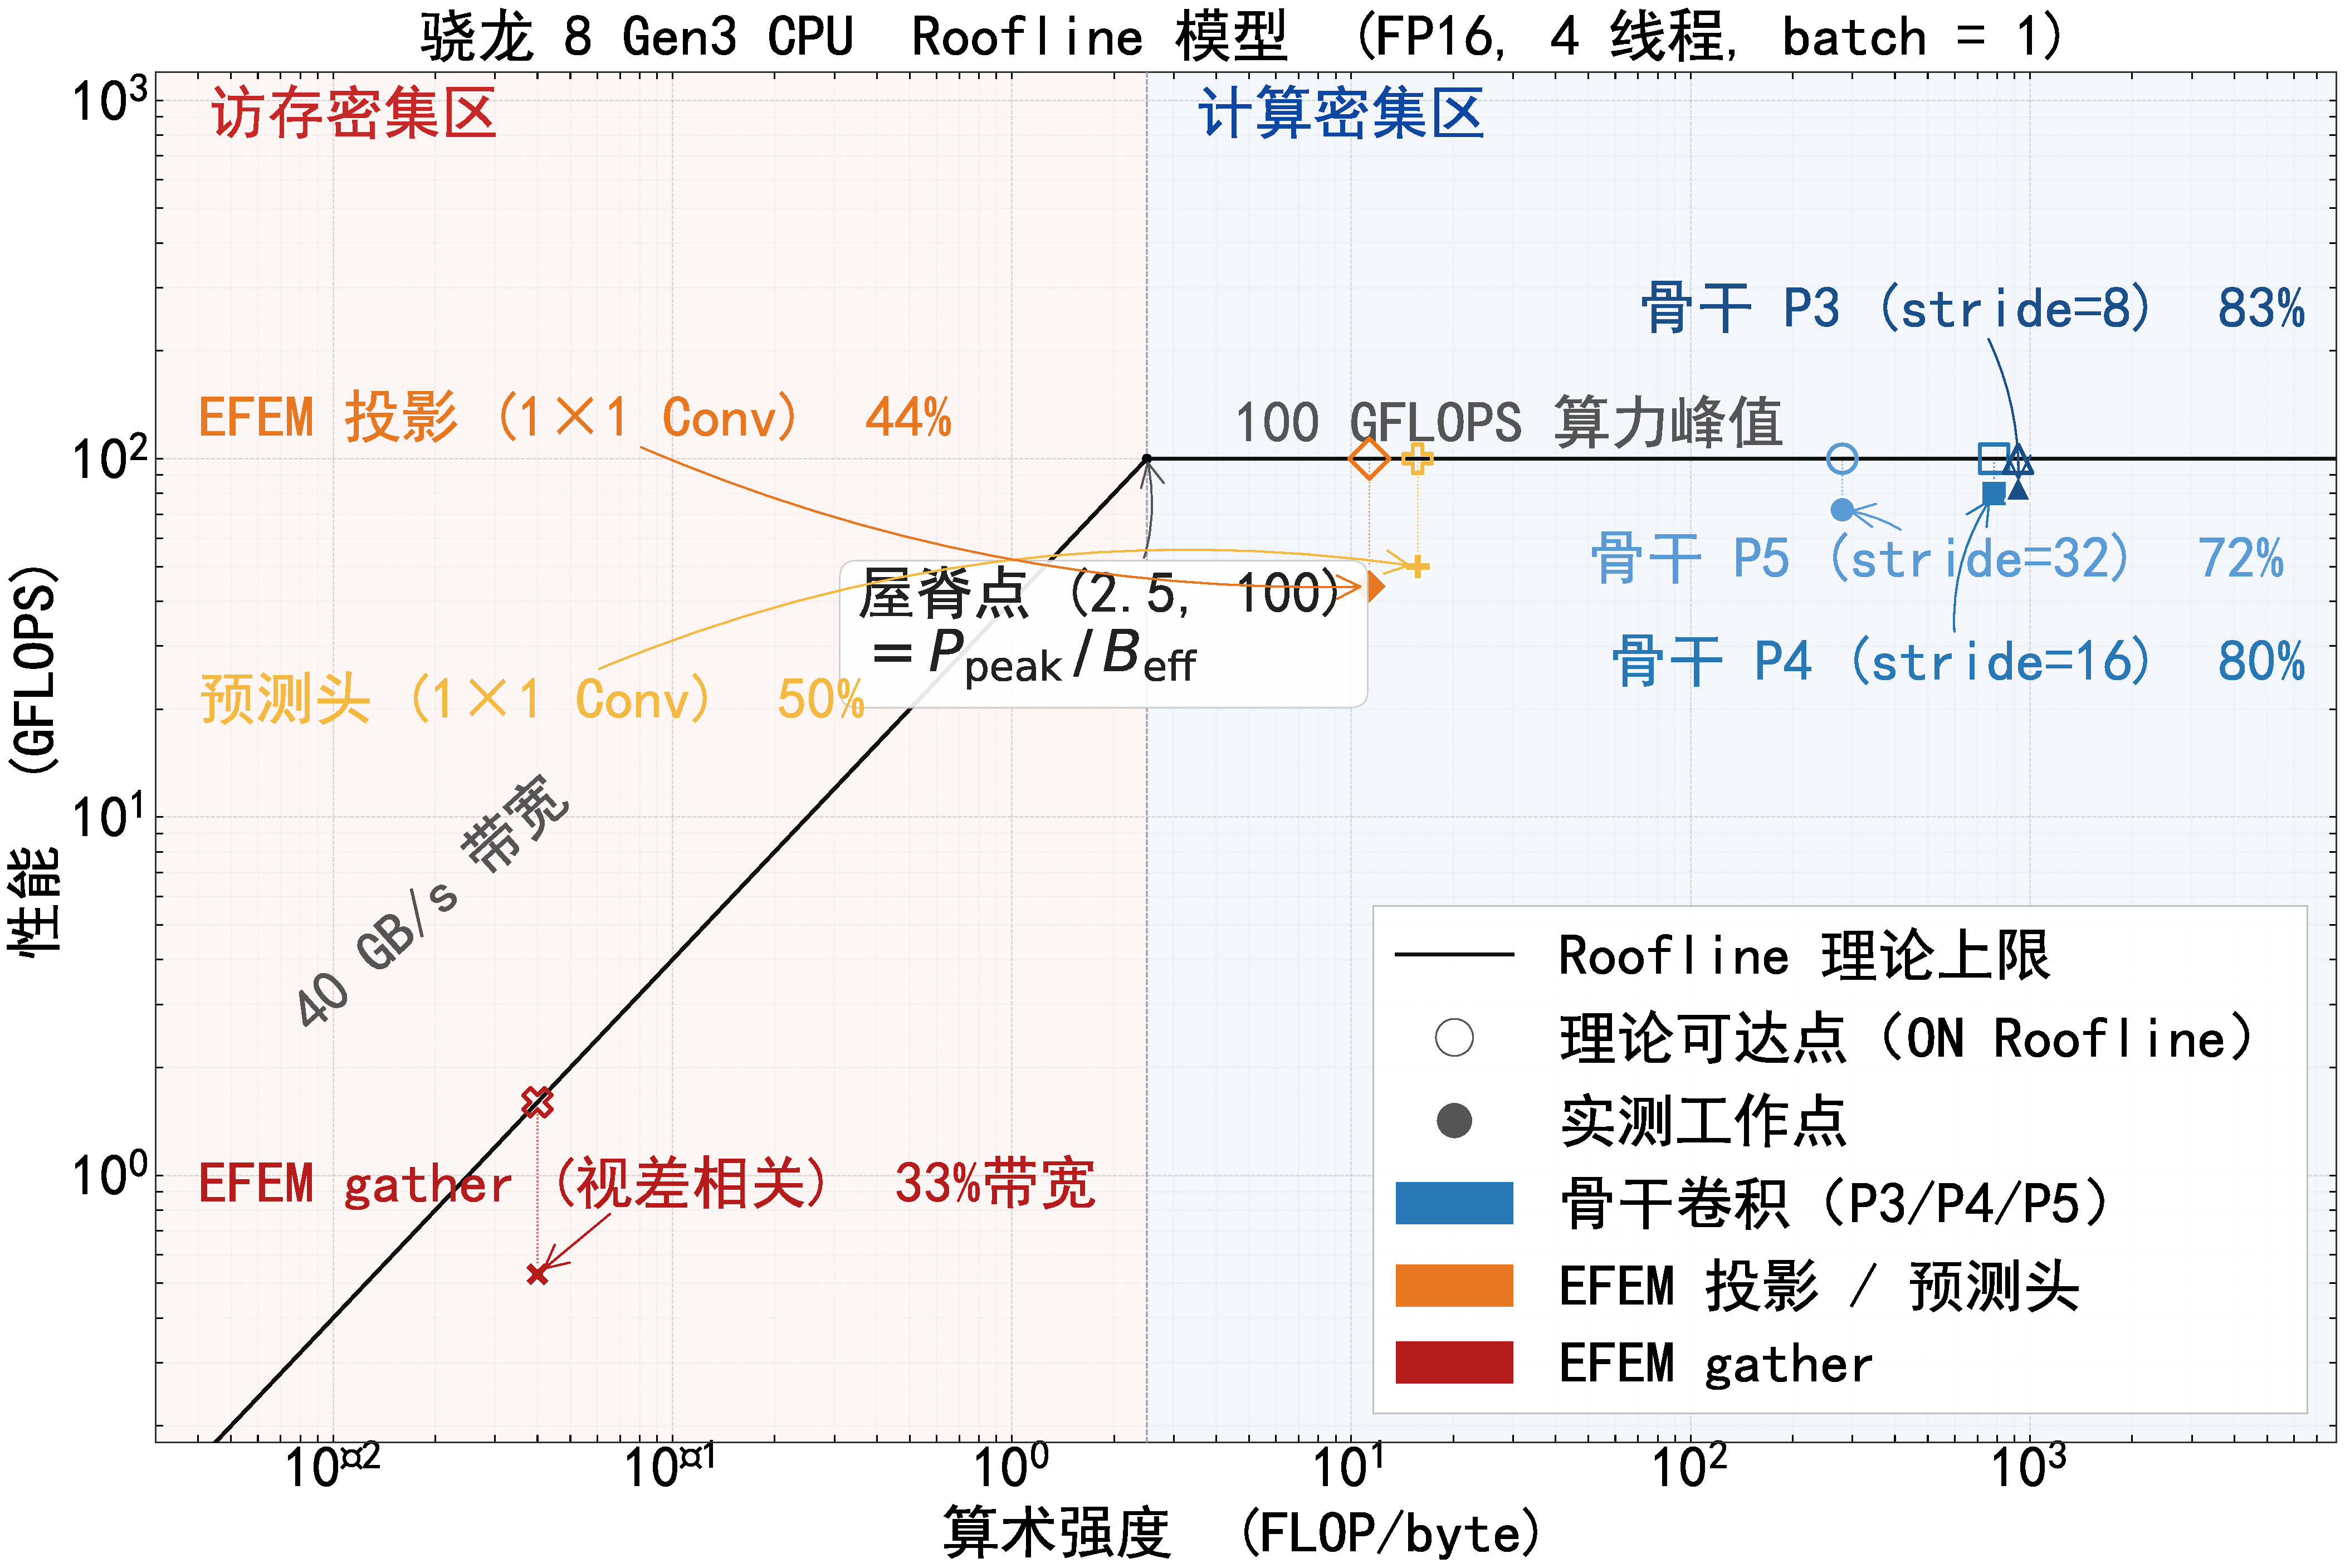
\includegraphics[width=\linewidth,height=3.6cm,keepaspectratio]{roofline.pdf}\\[1pt]
            \scriptsize 各模块 Roofline 分析（骨干为计算密集型，可受益于 INT8）\par}
            \vspace{2pt}
            \begin{exampleblock}{}
                \scriptsize 骨干 AI $\gg$ 脊点（2.5\,FLOP/byte）$\Rightarrow$ INT8 可显著加速\\
                EFEM gather AI $\approx$ 0.04 $\Rightarrow$ 内存受限，精度优先
            \end{exampleblock}
        \end{column}
        \begin{column}{0.47\textwidth}
            \scriptsize\textbf{逐层量化敏感性分析（单独替换为 INT8）}
            \vspace{2pt}
            \begin{table}
                \centering
                \scriptsize
                \setlength{\tabcolsep}{2pt}
                \renewcommand{\arraystretch}{1.05}
                \begin{tabular}{lcc}
                    \toprule
                    模块 & $\Delta$MPJPE & 决策 \\
                    \midrule
                    骨干卷积权重（主） & $+1.8$ & INT8 \\
                    骨干卷积权重（辅） & $+1.4$ & INT8 \\
                    EFEM 投影权重 & $+2.1$ & INT8 \\
                    EFEM 注意力激活 & $+6.8$ & \textcolor{red}{FP32} \\
                    热力图头输出 & $+3.2$ & \textcolor{red}{FP32} \\
                    置信头输出 & $+4.1$ & \textcolor{red}{FP32} \\
                    DWT 输入/输出 & $+7.3$ & \textcolor{red}{FP32} \\
                    \bottomrule
                \end{tabular}
            \end{table}
            \vspace{2pt}
            \begin{alertblock}{}
                \scriptsize 阈值：$\Delta E \leq 2.5$\,mm → INT8；$\Delta E \geq 5.0$\,mm → FP32 保护
            \end{alertblock}
        \end{column}
    \end{columns}
\end{frame}

%% ---- 量化 slide 3/4 ----
\begin{frame}[shrink=5]{混合精度量化方案设计}
    \begin{columns}[T]
        \begin{column}{0.50\textwidth}
            {\centering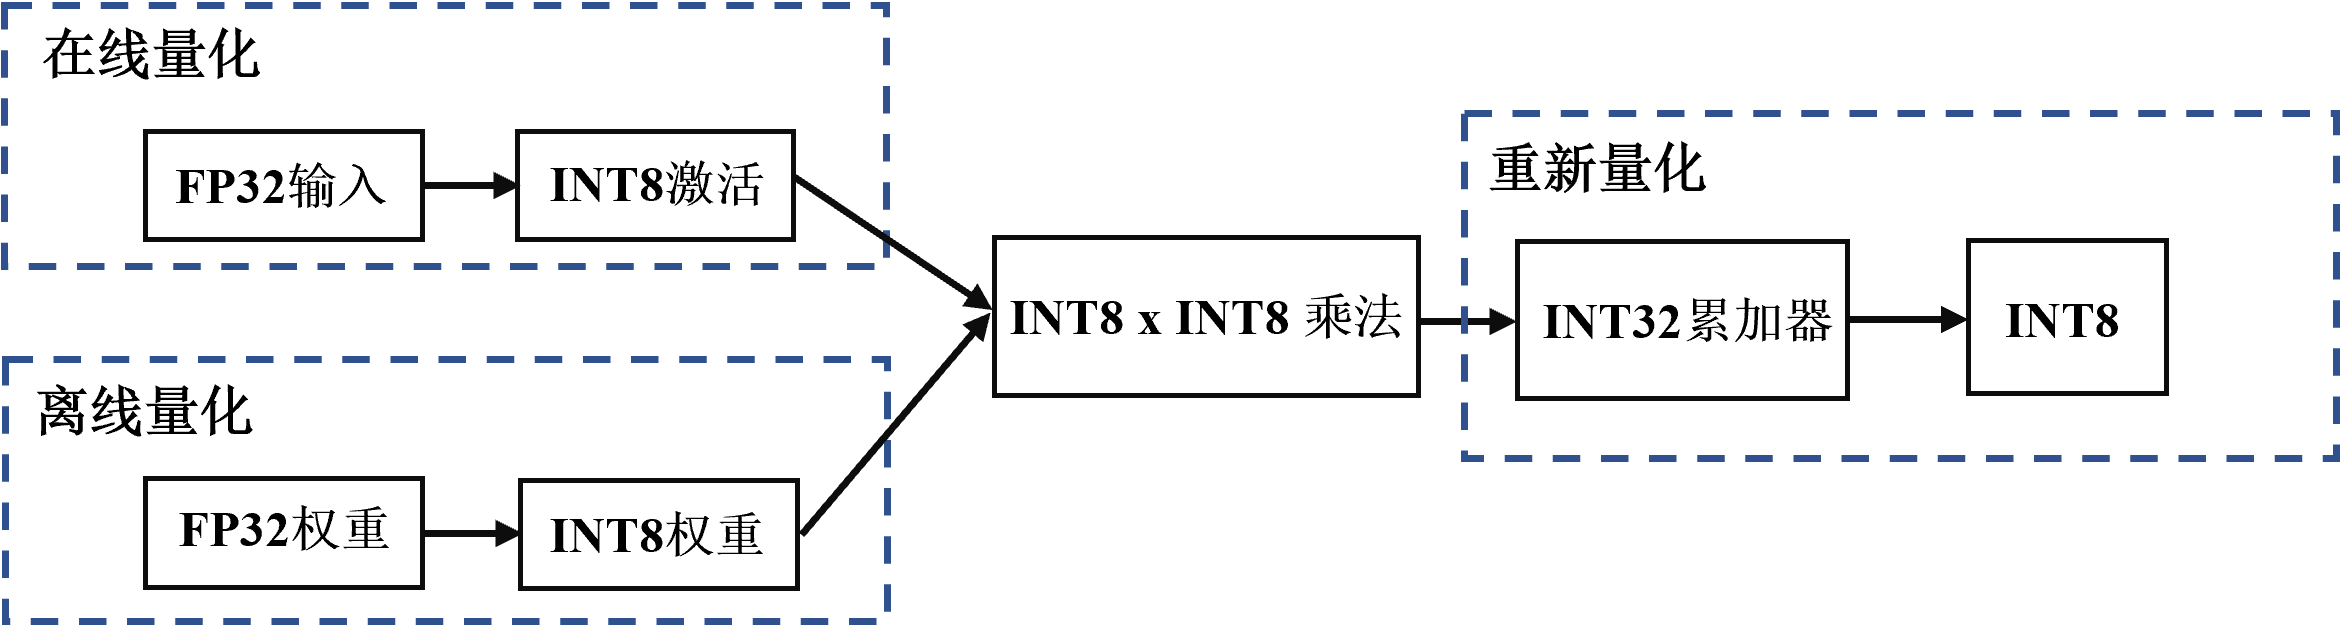
\includegraphics[width=\linewidth,height=4.8cm,keepaspectratio]{INT8QuantPipine.png}\\[2pt]
            \scriptsize INT8 量化推理流程（权重+激活同步量化，INT32 累加后重量化）\par}
            \vspace{4pt}
            \begin{block}{\small PTQ 部署流程}
                \scriptsize
                \textbf{①} PyTorch 训练模型\\[2pt]
                \textbf{②} ONNX 导出（opset 11）\\[2pt]
                \textbf{③} mnnconvert + 直方图-KL 校准（256张）\\[2pt]
                \textbf{④} MNN 混合精度 engine 推理
            \end{block}
        \end{column}
        \begin{column}{0.47\textwidth}
            \footnotesize\textbf{分层精度分配方案}
            \vspace{2pt}
            \begin{table}
                \centering
                \scriptsize
                \setlength{\tabcolsep}{2pt}
                \renewcommand{\arraystretch}{1.05}
                \begin{tabular}{lccr}
                    \toprule
                    模块 & 精度 & $\Delta E$(mm) & 占比 \\
                    \midrule
                    骨干 Conv & INT8 & $+1.6$ & \multirow{2}{*}{99.1\%} \\
                    EFEM 投影权重 & INT8 & $+2.1$ & \\
                    \midrule
                    EFEM 注意力激活 & FP32 & $+6.8$ & \multirow{3}{*}{0.9\%} \\
                    热力图/置信头 & FP32 & $+3.7$ & \\
                    DWT 求解器 & FP32 & $+7.3$ & \\
                    \bottomrule
                \end{tabular}
            \end{table}
            \vspace{3pt}
            \begin{alertblock}{\small 量化决策准则}
                \scriptsize
                $\Delta E{\leq}2.5$\,mm $\Rightarrow$ \textbf{INT8}（计算密集，可加速）\\
                $\Delta E{\geq}3.0$\,mm $\Rightarrow$ \textbf{FP32}（精度敏感，须保护）
            \end{alertblock}
        \end{column}
    \end{columns}
\end{frame}

%% ---- 量化 slide 4/4 ----
\begin{frame}[shrink=5]{量化实验结果（Xiaomi 14）}
    \begin{table}
        \centering
        \footnotesize
        \setlength{\tabcolsep}{4pt}
        \renewcommand{\arraystretch}{1.15}
        \begin{tabular}{lccccc}
            \toprule
            配置 & MPJPE & $\Delta$MPJPE & 延迟 & 加速比 & 模型大小 \\
            \midrule
            FP32 & 158.6 & -- & 208.7\,ms & 0.56$\times$ & 46.8\,MB \\
            FP16 基线 & 158.6 & -- & 116.0\,ms & 1.00$\times$ & 23.4\,MB \\
            INT8 全量 & 172.0 & $+13.4$ & \textbf{67.8\,ms} & \textbf{1.71$\times$} & \textbf{11.7\,MB} \\
            \textbf{本文混合精度} & \textbf{160.8} & \textbf{+2.2} & \textbf{72.3\,ms} & \textbf{1.60$\times$} & \textbf{15.2\,MB} \\
            \bottomrule
        \end{tabular}
    \end{table}
    \vspace{3pt}
    \begin{columns}[T]
        \begin{column}{0.50\textwidth}
            \footnotesize\textbf{保护层消融实验}
            \vspace{2pt}
            \begin{table}
                \centering
                \scriptsize
                \setlength{\tabcolsep}{3pt}
                \renewcommand{\arraystretch}{1.1}
                \begin{tabular}{lcc}
                    \toprule
                    变体 & MPJPE & $\Delta$ \\
                    \midrule
                    本文混合精度 & 160.8 & -- \\
                    EFEM 注意力 → INT8 & 167.3 & $+6.5$ \\
                    热力图/置信头 → INT8 & 163.5 & $+2.7$ \\
                    DWT → INT8 & 168.2 & $+7.4$ \\
                    三者全 INT8 & 172.4 & $+11.6$ \\
                    \bottomrule
                \end{tabular}
            \end{table}
        \end{column}
        \begin{column}{0.47\textwidth}
            \begin{exampleblock}{\small 核心收益}
                \footnotesize
                \begin{itemize}
                    \item 混合精度 vs FP16：\textbf{1.60$\times$ 加速}
                    \item 模型大小 23.4→\textbf{15.2\,MB}（↓\textbf{35\%}）
                    \item 精度损失 $\Delta$MPJPE 仅 \textbf{+2.2\,mm}
                \end{itemize}
            \end{exampleblock}
            \vspace{4pt}
            \begin{alertblock}{\small 对比 INT8 全量}
                \footnotesize
                精度损失从 $+13.4$\,mm 降至 \textbf{+2.2\,mm}\\
                速度仅略降：1.71$\times$ → \textbf{1.60$\times$}\\
                \textbf{精度–速度最优权衡点}
            \end{alertblock}
        \end{column}
    \end{columns}
\end{frame}

%% ---- 量化 slide 补充：Jetson ----
\begin{frame}[shrink=5]{Jetson AGX Xavier 平台验证}
    \begin{columns}[T]
        \begin{column}{0.48\textwidth}
            {\centering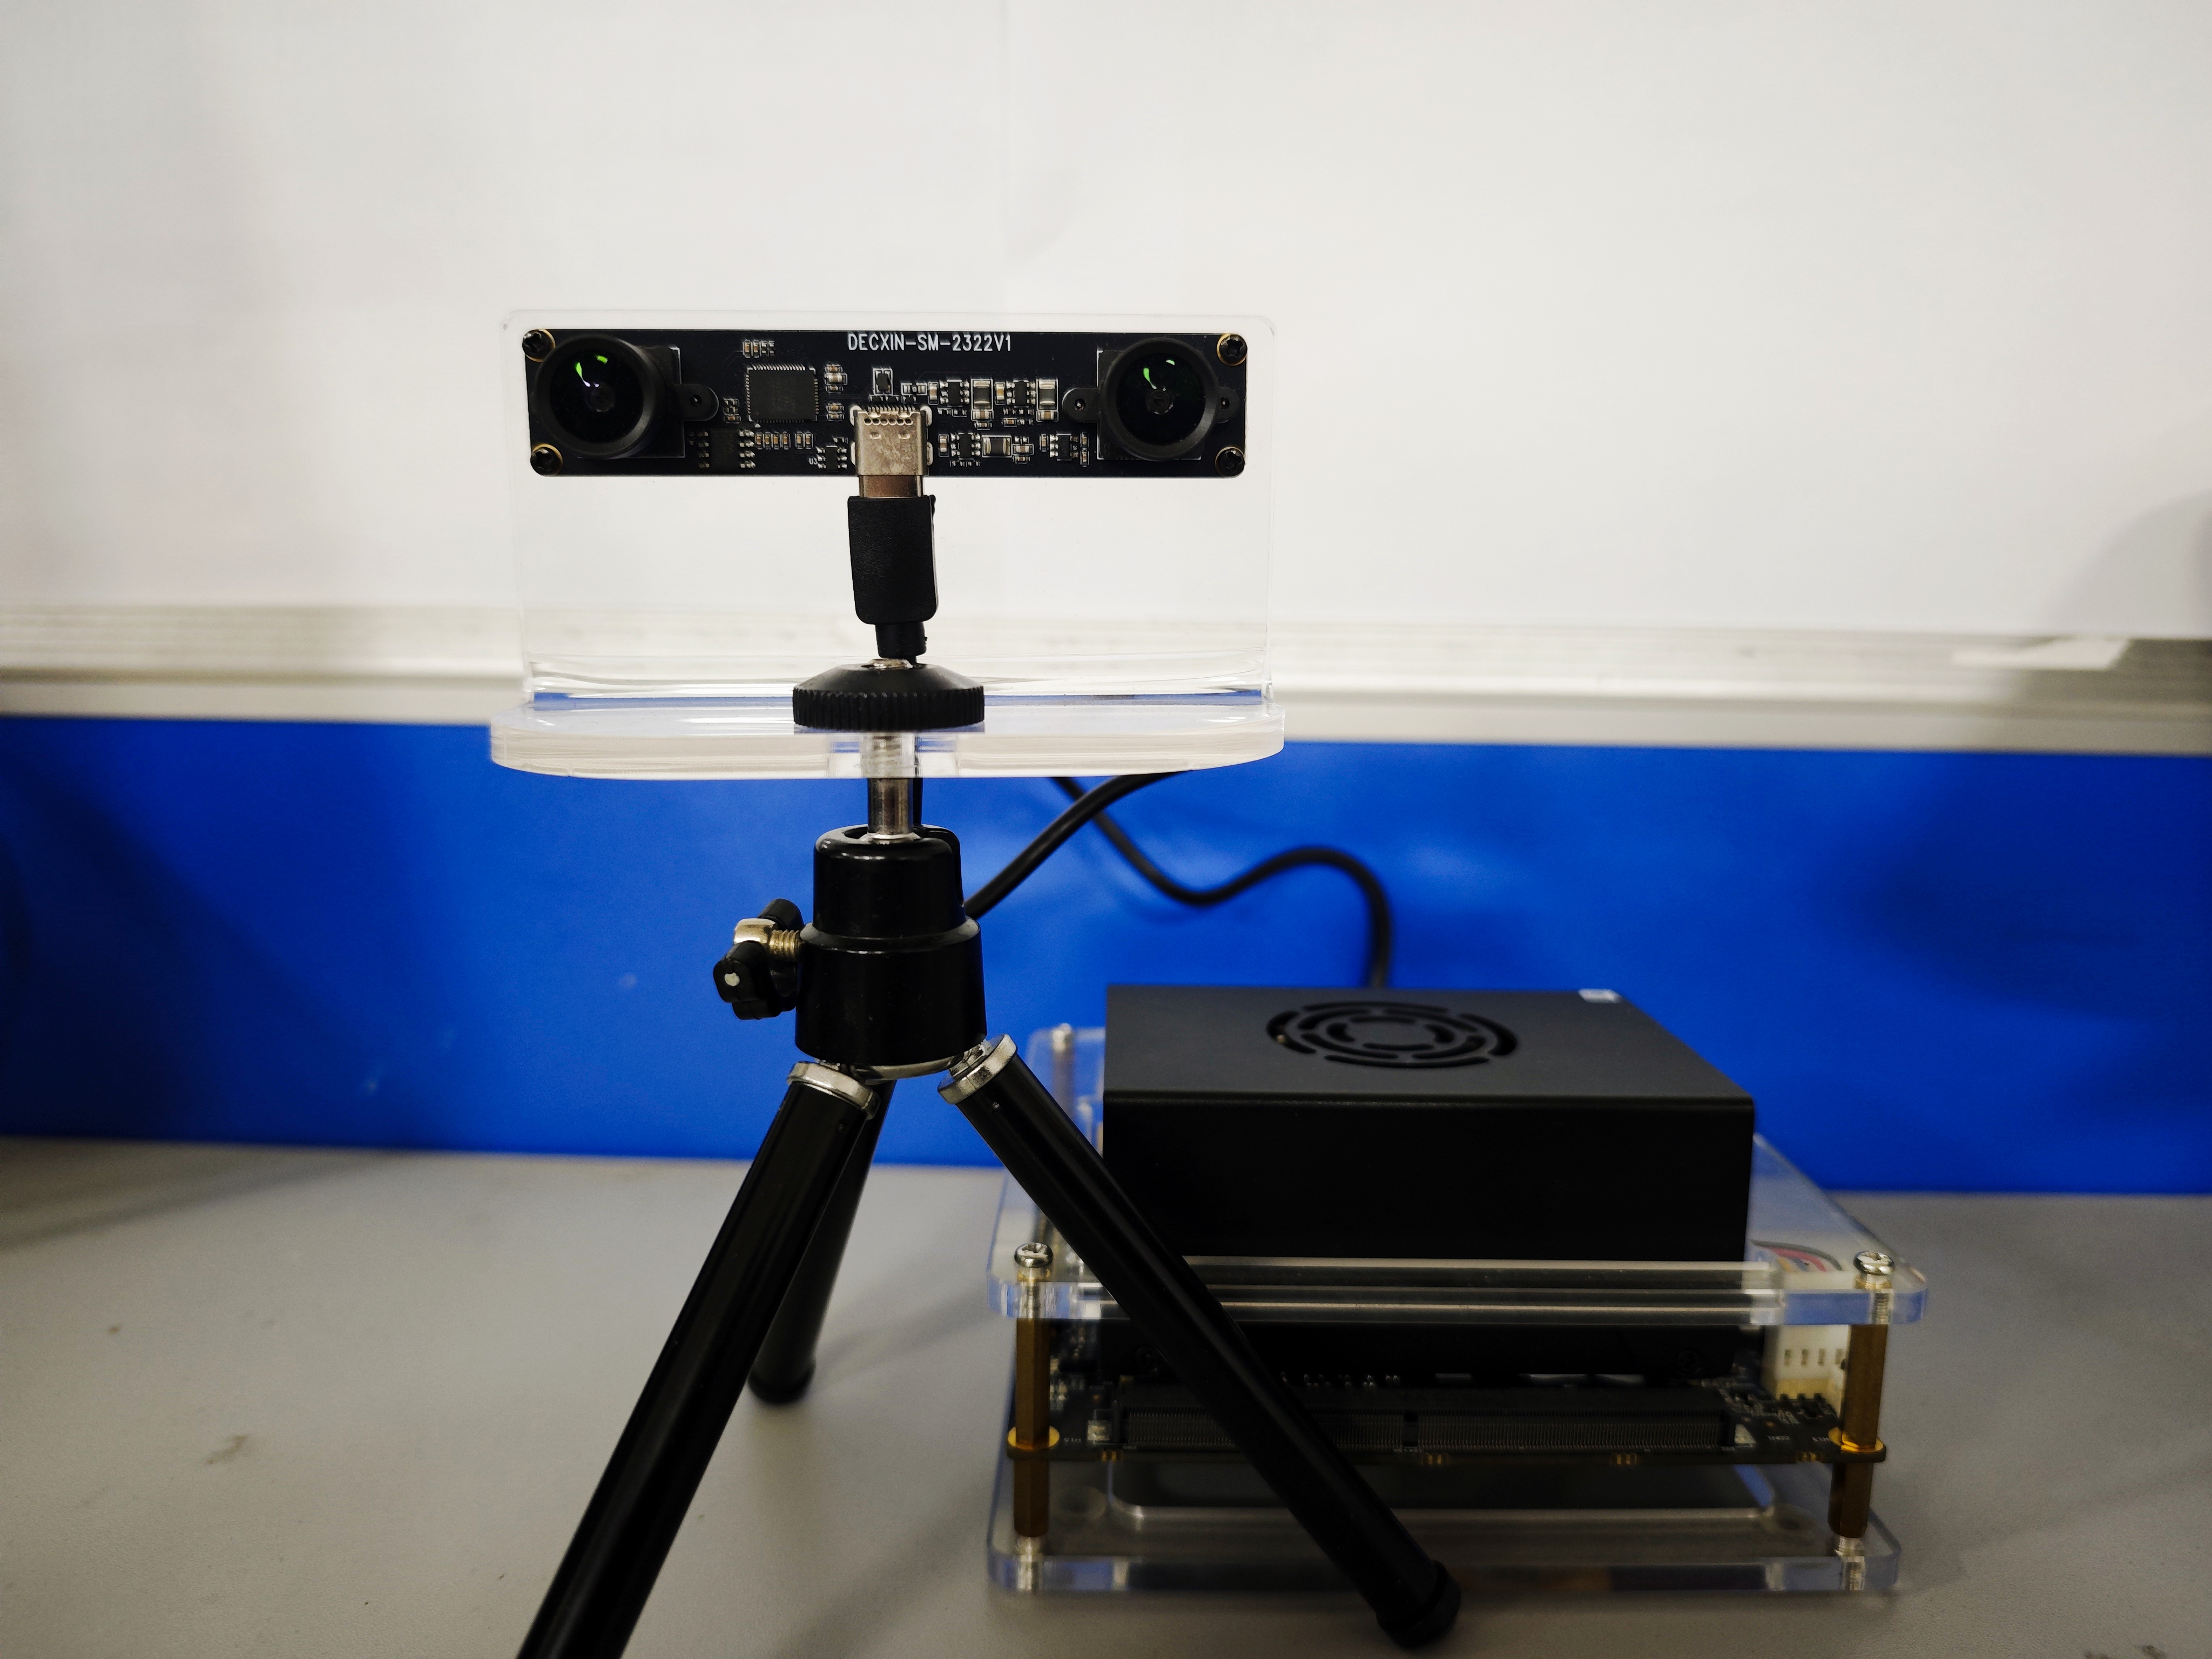
\includegraphics[width=\linewidth,height=3.2cm,keepaspectratio]{PhysicalSystem.jpg}\\[2pt]
            \footnotesize 实物部署系统\par}
        \end{column}
        \begin{column}{0.48\textwidth}
            {\centering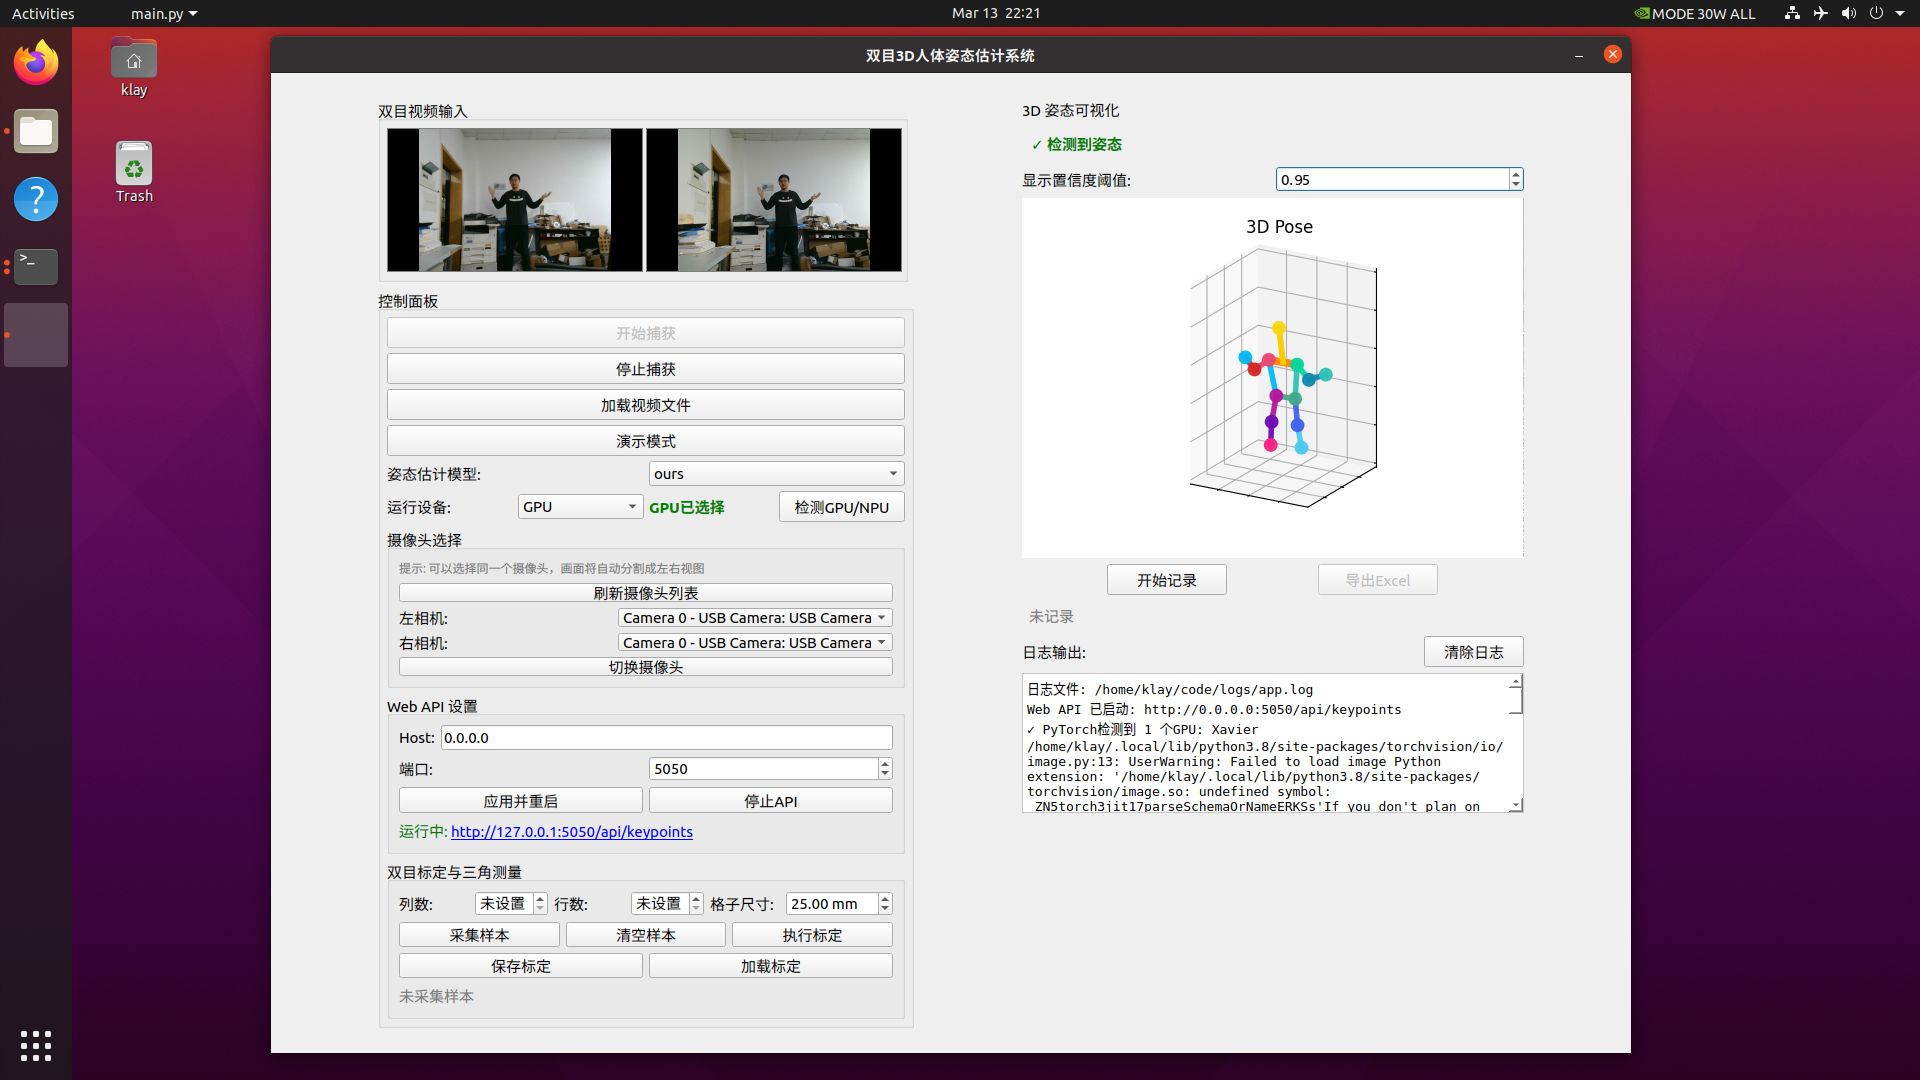
\includegraphics[width=\linewidth,height=3.2cm,keepaspectratio]{Screenshot.png}\\[2pt]
            \footnotesize Jetson 平台运行界面\par}
        \end{column}
    \end{columns}
    \vspace{4pt}
    \begin{table}
        \centering
        \footnotesize
        \renewcommand{\arraystretch}{1.1}
        \setlength{\tabcolsep}{5pt}
        \begin{tabular}{lcccc}
            \toprule
            精度 & MPJPE & 延迟 & 显存 & 能耗 \\
            \midrule
            FP16 & 158.6 & 25.4\,ms & 412\,MB & 0.441\,J \\
            INT8 & 172.0 & 15.8\,ms & 236\,MB & 0.299\,J \\
            \textbf{混合精度} & \textbf{160.8} & \textbf{20.6\,ms} & \textbf{298\,MB} & \textbf{0.375\,J} \\
            \bottomrule
        \end{tabular}
    \end{table}
    \vspace{2pt}
    \begin{center}
        \footnotesize 混合精度 engine：\textbf{48.5 FPS}，$\Delta$MPJPE = +2.2\,mm，0.375\,J/frame
    \end{center}
\end{frame}


%% ========================================
\section{总结与展望}
%% ========================================

\begin{frame}{总结}
    \begin{block}{三项主要贡献}
        \small
        \begin{enumerate}
            \item \textbf{轻量化端到端双目框架}\\
                非对称骨干 + EFEM + DWT，参数量 11.70\,M，FLOPs 13.93\,G\\
                RT-Pose MPJPE \textbf{158.6\,mm}，较最优双目基线↓38.2\,mm
            \vspace{2pt}
            \item \textbf{零样本泛化 \& 多人实时}\\
                RT-Pose→MADS 不微调：\textbf{33.68\,mm}，优于全部对比方法\\
                1\textasciitilde10 人时延近似不变（116.0\,ms → 117.3\,ms）
            \vspace{2pt}
            \item \textbf{硬件感知混合精度部署}\\
                Xiaomi 14：1.60$\times$ 加速，$\Delta$MPJPE = +2.2\,mm\\
                Jetson AGX Xavier：\textbf{48.5 FPS}，298\,MB，0.375\,J/frame
        \end{enumerate}
    \end{block}
\end{frame}

\begin{frame}{展望}
    \begin{itemize}
        \item \textbf{跨硬件部署}：Android NPU / iOS Core ML 等平台适配
        \vspace{6pt}
        \item \textbf{复杂场景鲁棒性}：极端遮挡、小视差、标定漂移的几何先验增强
        \vspace{6pt}
        \item \textbf{量化感知训练}：QAT 与视频时序双目推理
        \vspace{6pt}
        \item \textbf{双目数据集建设}：室外多基线、复杂光照场景数据补充
    \end{itemize}
\end{frame}

\begin{frame}
    \begin{center}
        {\Huge\calligra 感谢各位老师的聆听！}\\[1.5em]
        {\large 敬请批评指正}
    \end{center}
\end{frame}

\end{document}
